\documentclass{trkut}% Reaalkooli vormistus. Muidu "report" või "article".
\usepackage[style=trkut]{biblatex}% Kasutatud kirjanduse genereerimine
\usepackage{listings}
\usepackage{mleftright, braket}
\addbibresource{viited_kaarel_kivisalu.bib}% Viidete info fail
\defbibheading{bibliography}{\addchap{#1}}% Lisame kasutatud materjalid sisukorda

\pealkiri{Gravitatsiooni mõju osakeste süsteemi soojusmahtuvusele erinevates potentsiaalides}
\autor{Kaarel Kivisalu}
\klass{11. a}
\juhendaja{prof Jaan Kalda \\ õp Toomas Reimann}
\toggletrue{mitujuhendajat}% Uncomment kui on mitu juhendajat

\DeclareMathOperator{\tr}{tr}
\DeclareMathOperator{\erf}{erf}
\NewDocumentCommand{\op}{o m}{\IfNoValueTF{#1}{\hat{#2}}{\hat{#2}^{#1}}}
\renewcommand\bra[1]{{\langle{#1}|}}
\renewcommand\ket[1]{{|{#1}\rangle}}
\renewcommand\Bra[1]{\mleft\langle#1\mright|}
\renewcommand\Ket[1]{\mleft|#1\mright\rangle}
\renewcommand\braket[1]{\langle{#1}\rangle}
\reversemarginpar

\lstdefinelanguage{Maxima}{
keywords={sum, subst, diff, plot3d, log},
sensitive=true,
}

\begin{document}
\maketitle% Tiitelleht
\tableofcontents% Sisukord

\addchap{Tähiste loetelu}
\begin{tabular}{l l}
    $T$ & absoluutne temperatuur \\
    $\op{H}$ & hamiltoniaani operaator \\
    $x/\op{x}$ & ruumikoordinaat/asukohaoperaator \\
    $\braket{\op{O}}$ & operaatori $\op{O}$ ooteväärtus \\
    $\op{\rho}$ & tihedusmaatriks \\
    $Z$ & statistiline summa \\
    $\bra{a}$ & bra ehk veeruvektor \\
    $\ket{a}$ & ket ehk reavektor \\
    $\overline{a}$ & $a$ keskväärtus \\
    $\psi$ & lainefuntsioon \\
    $C$ & soojusmahtuvus \\
    $m$ & mass \\
    $g$ & gravitatsioonivälja tugevus \\
    $E$ & energia \\
    $V$ & potentsiaal \\
    $\omega$ & nurksagedus \\
    $N$ & summeerimisel kasutatud liikmete arv \\
    $\hbar$ & taandatud Plancki konstant \\
    $k_B$ & Boltzmanni konstant \\
    $i$ & imaginaarühik \\
\end{tabular}


\addchap{Sissejuhatus}
\nummerdame% See käsk peab olema õigeks nummerdamiseks kohe peale sissejuhatust
Kehade soojusmahtuvust on põhjalikult uuritud nii klassikaliselt kui ka kvantmehaaniliselt.
On olemas head soojusmahtuvuse mudelid tahkiste ja gaaside jaoks.
Ometi tõi välja I rahvusvahelise füüsikaolümpiaadi 1967. aasta ülesanne efekti, mida ei oldud varem põhjalikult uuritud.
Olümpiaadiülesanne oli järgmine \parencite[6]{ipho67}:

\textit{Kaks homogeenset ühesugust kera on sama algtemperatuuriga. Üks kera on liikumatult horisontaalse tasandil, teine ripub niidi küljes. Mõlemale kerale antakse võrdne soojushulk. Kas kerade lõpptemperatuur on sama või mitte? Soojuskadudega mitte arvestada.}

Selle ülesande algses lahenduses leiti, et enamiku materjalide jaoks on on horisontaalsel tasandil oleva kera soojusmahtuvus on suurem riputatud kera omast.
St, et tasandil oleva kera temperatuur on pärast soojushulga andmist väiksem.
Hiljuti leiti Palma ja Sormani poolt, et algne lahendus rikub termodünaamika II seadust.
Nad pakkusid välja kaks alternatiivset lahendust kasutades statistilist mehaanikat ja klassikalist termodünaamikat.
Mõlema lahendusga saadi sama tulemus ja seoti omavahel kera soojusmahtuvuse ja lineaarse soojuspaisumisteguri.

Käesolevas töös uuritakse konkreetsete potentsiaalide korral konstantse gravitatsioonvälja mõju kerale sarnasele, kuid lihtsustatud süsteemi soojusmahtuvusele.
Täpsemalt vaatatakse süsteemi, kus kõik osakesed peale ühe on fikseeritud ja see osake saab liikuda ainult ühes dimensioonis.
Konstantse gravitatsioonivälja potentsiaal on lineaarne ja selle saab liita süsteemi potentsiaalile.
Käesolevas töös tahetakse leida seas süsteemi potentsiaali ja soojusmahtuvuse vahel.

Töös analüüsitakse kuuphäiritusega harmoonilise ostsillaatori potentsiaali häirituse meetodil ja tükati sirgetest koosnevat potentsiaali kvaasi-klassikaliselt.
Harmoonilise ostsillaatori potentsiaal on valitud, kuna selline potentsiaal on tüüpiliselt potentsiaalimiinimumide ümber.
Laialdaselt kasutatakse harmoonilise ostsillaatori potentsiaali näiteks kaheaatomilise molekuli lihtsa mudelina.
Tükati sirgetest koosnev potentsiaal on valitud selle arvutusliku lihtususe tõttu.

%Varem on uuritud gravitatsiooni mõju metallkera soojusmahtuvusele Palma ja Sormani poolt \parencite{palma15}.
%Leiti üldine seos soojusmahtuvuse, temperatuuri, gravitatsioonivälja tugevuse ja lineaarse soojuspaisumisteguri vahel.
%Saadud tulemust on eksperimentaalselt väga raske kinnitada, kuna gravitatsiooni mõju on väga väike.
%Konkreetsete potentsiaalide läbivaatamine tõstaks ka varem leitud mudeli usaldusväärsust.

Uurimistöö hüpoteesiks on, et sõltuvalt valitud potentsiaalist võib gravitatsiooniväli nii tõsta kui ka langetada keha soojusmahtuvust.

Uurimistöö on jaotatud kahte ossa.
Esimeses osas tutvustatakse varasemaid tulemusi kera soojusmahtuvuse kohta ja potentsiaalide analüüsis kasutatavaid meetodeid.
Teises osas kirjeldatakse töös kasutatavat mudelit ja analüüsitakse erinevaid potentsiaale.



\chapter{Ülevaade kirjandusest ja teooriast}

%Siin peatükis on välja toodud olümpiaadiülesande algne lahendus ja põhjendatud, miks see rikub termodünaamika II seadust (osad \ref{algne} ja \ref{rikub}).
%Samuti on välja toodud alternatiivse lahendusega saadud tulemus (vt võrrand \eqref{palmasor}).
\section{Olümpiaadiülesande algne lahendus} \label{algne}

Algne lahendus põhineb soojuspaisumisega seotud erinevustel. Tasapinnal olevale kerale $A$ soojust andes see paisub ja selle massikese tõusej. Järelikult peab osa kerale A antavast soojushulgast kuluma kera massikeskme gravitatsioonilise potentsiaalse energia tõstmiseks, mis langetab kera temperatuuri. Vastupidiselt, rippuva kera $B$ massikese langeb soojuspaisumise tõttu ja energiat saadakse juurde, mis tõstab kera B temperatuuri. \parencite[6-7]{ipho67}

Olgu kerade soojusmahtuvus $C_0$ gravitatsioonivälja puudumisel. Algse lahenduse järgi, kui kera A soojendatakse, siis selle massikese tõuseb $dR=\alpha R \, dT$ võrra, kus $dT$ on temperatuuri tõus, $\alpha$ on soojuspaisumistegur ja $R$ on kera raadius. Kera saab juurde potentsiaalse energia $d\Phi = mg \, dR$, kus $m$ on keha mass ja $g$ on gravitatsioonivälja tugevus. Järelikult, kui soojushulk \(\delta Q\) antakse süsteemile, siis saadakse, et \parencite[2-3]{palma15}
\begin{equation}
    \delta Q = C_0 \, dT + mg \, dR = C_0 \, dT + mg\alpha R \, dT = (C_0 +  mg\alpha R) dT.
\end{equation}
See on ekvivalentne väitega, et kera \(A\) soojusmahtuvus
\begin{equation}
    C_A = C_0 + mg\alpha R.
\end{equation}
Analoogselt saadakse, et kera \(B\) soojusmahtuvus
\begin{equation}
    C_B = C_0 - mg\alpha R.
\end{equation}
Enamiku materjalide korral on \(\alpha > 0\), millest tulenevalt \(C_A>C_B\). Järelikult on tavapärase lahenduse kohaselt kera \(A\) lõpptemperatuur madalam kera \(B\) lõpptemperatuurist.

\section{Algne lahendus rikub termodünaamika II seadust} \label{rikub}

Algses lahenduses kaudselt eeldatakse, et keha siseenergia \(U\) ja raadius \(R\) sõltuvad ainult temperatuurist \(T\), mitte aga raskuskiirendusest \(g\).
Vaadeldakse järgnevat tsüklit: kera asub horisontaalsel külmal tasandil temperatuuriga \(T_1\); kera ühendatakse soojema reservuaariga, mille temperatuur \(T_2=T_1+dT>T_1\); kera riputatakse nööri külge ja horisontaalne tasand eemaldatakse; kera ühendatakse külma reservuaariga, mille temperatuur on \(T_1\).
Selle protsessi kasutegur on tehtud töö ja neeldunud soojushulga suhe ning avaldub kujul \parencite[3-5]{palma15}
\begin{equation}
    \eta = \frac{2mg\alpha R}{C_0+mg\alpha R}.
\end{equation}
Kasutegur \(\eta\) ei sõltu \(dT\) suurusest. Termodünaamika teist seadust saab sõnastada järgnevalt: iga tsükkel, mis töötab ainult temperatuuride \(T_1\) ja \(T_2\) vahemikus ei saa olla efektiivsem Carnot' tsüklist, mis töötab samade temperatuuride juures. Carnot' tsükli efektiivsus on \parencite[3-5]{palma15}
\begin{equation}
    \eta_{Carnot'} = \frac{dT}{T_2}.
\end{equation}
Järelikult, kui \(dT\) on piisavalt väike, siis on keraga tsükli kasutegur suurem Carnot' tsükli kasutegurist. Teisisõnu rikub algne lahendus termodünaamika II seadust.

%\begin{figure}[h]
%    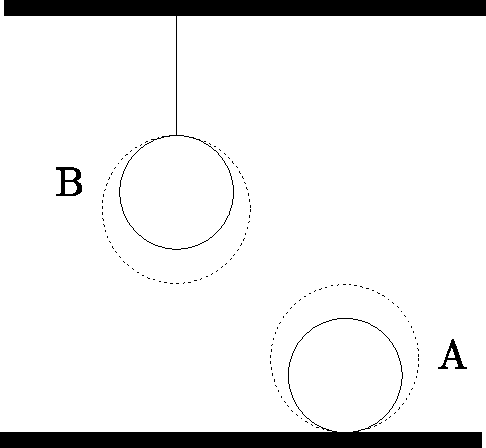
\includegraphics[width=0.5\textwidth]{joonis1.pdf}
%    \caption{Probleemi ülesehitus}
%    \allikas{\protect\cite[15]{palma15}}
%    \label{iphojoonis}% Selle järgi viidatakse, see rida peab olema pärast \caption
%\end{figure}

%\section{Schrödingeri võrrand}
%
%Ajast sõltumatu Schrödingeri võrrand ühes dimensioonis avaldub kujul \cite{griffiths05}
%\begin{equation}
%    \op{H} \Psi = E \Psi,
%\end{equation}
%kus \(E\) on süsteemi koguenergia ja
%\begin{equation}
%    \op{H}=-\frac{\hbar^2}{2m}\frac{d^2}{dx^2}+V(x).
%\end{equation}

\section{Kvantmehaaniline statistiline mehaanika}

Kvantmehaanilises statistilises mehaanikas on mugav kasutada tihedusmaatriksit (ingl \textit{density matrix}) $\op{\rho}$ kvantmehaanilise operaatori ooteväärtuse (ingl \textit{expectation value}) leidmiseks.
Tihedusmaatriks on defineeritud järgnevalt \parencite[172]{kardar07}:
\begin{equation}
    \op{\rho}(t) \equiv \sum_j p_j \ket{\Psi_j(t)} \bra{\Psi_j(t)},
\end{equation}
kus $\sum_j p_j=1$, $p_j > 0$ ja $\ket{\Psi_j}$ on puhas kvantolek (ingl \textit{pure quantum state}).
See kujutab segakvantolekut (ingl \textit{mixed quantum state}), kus tõenäosusega $p_j$ on süsteem puhtas kvantolekus $\ket{\Psi_j}$.
Selles formalismis avaldub kvantmehaanilise operaatori ooteväärtuse ansambli keskväärtus järgnevalt \parencite[172]{kardar07}:
\begin{equation}
    \overline{\braket{\op{O}}}=\tr(\op{\rho}\op{O}),
    \label{ootev}
\end{equation}
kus jälg (ingl \textit{trace}) $\tr(\op{A}) \equiv \sum_n \braket{n|\op{A}|n}$. %\footnote{\url{http://en.citizendium.org/wiki/Trace_\%28mathematics\%29} lõputu dimensioon converges} \parencite{viide}.
Kanoonilise ansambli\footnote{Ansambel, kus süsteem on soojuslikus tasakaalus fikseeritud temperatuuriga reservuaariga.} jaoks, mis on kvantmehaaniline ja diskreetne, avaldub kanooniline tihedusmaatriks järgnevalt \parencite[174]{kardar07}:
\begin{equation}
    \op{\rho}(\beta) = \frac{e^{-\beta \op{H}}}{Z(\beta)},
    \label{tihm}
\end{equation}
kus $\beta \equiv \frac{1}{k_B T}$, kus $T$ on absoluutne temperatuur ja $k_B$ on Boltzmanni konstant.
Kuna $\bra{\Psi_j}$ on normeeritud, siis
\begin{equation}
    \braket{1}=\tr(\op{\rho})=\sum_n \braket{n|\op{\rho}|n}=\sum_{n, j} p_j |\braket{n| \Psi_j}|^2=\sum_j p_j=1.
    \label{tihnorm}
\end{equation}
Võrranditest \eqref{tihm} ja \eqref{tihnorm} ning omadusest $\tr(c\op{A})=c\tr(\op{A})$ saadakse kvantmehaaniline statistiline summa $Z$, mis avaldub kujul
\begin{equation}
    Z=\tr(e^{-\beta \op{H}})=\sum_n e^{-\beta \op{H}}.
    \label{part}
\end{equation}
Kasutades võrrandeid \eqref{ootev}, \eqref{tihm} ja \eqref{part} saadakse hamiltoniaani $\op{H}$ keskmine ooteväärtus
\begin{equation}
    \overline{\braket{\op{H}}}=\tr(\op{\rho}\op{H})=\frac{\tr{\op{H}e^{-\beta \op{H}}}}{Z}= -\frac{\partial \ln Z}{\partial \beta}.
    \label{keskham}
\end{equation}
Hamiltoniaani keskmist ooteväärtust võib mõista kui süsteemi energiat. Kuna ollakse huvitatud temperatuuri muutusest, kui süsteemile antakse mingi energiahulk, siis on kasulik defineerida soojusmahtuvus kui $\overline{\braket{\op{H}}}$ osatuletis $T$ järgi:
\begin{equation}
    C = \frac{\partial \overline{\braket{\op{H}}}}{\partial T}.
    \label{soojuham}
\end{equation}
Kombineerides võrrandeid \eqref{keskham} ja \eqref{soojuham} saadakse, et
\begin{equation}
    C = k_B T^2 \frac{\partial^2 \ln Z}{\partial \beta^2}
    \label{mahtuvus}
\end{equation}

Kasutades selles osas saadud seoseid on võimalik leida kera soojusmahtuvuse sõltuvus gravitatsioonivälja tugevusest \parencite[10-13]{palma15}:
\begin{equation} \label{palmasor}
    \frac{\partial C(g,T)}{\partial g} = -mTY \left( \alpha^2 + \frac{\partial \alpha}{\partial T} \right),
\end{equation}
kus \(C\) on soojusmahtuvus, \(g\) on gravitatsioonivälja tugevus, \(m\) on kera mass, \(T\) on kera temperatuur, \(Y\) on massikeskme kõrgus, \(\alpha\) on lineaarne soojuspaisumistegur.


\section{Kvaasi-klassikaline lähendus}

\Huge
\textbf{Sissejuhatus teemale}
\normalsize

Ajast sõltumatu Schrödingeri võrrandi ühes dimensioonis
\begin{equation}
    -\frac{\hbar^2}{2m}\frac{d^2\psi(x)}{dx^2}+V(x)\psi=E\psi
\end{equation}
saab ümber kirjutada järgnevalt:
\begin{equation}
    \frac{d^2 \psi(x)}{dx^2}= - \frac{p(x)^2}{\hbar^2}\psi,
\end{equation}
kus
\begin{equation} \label{klassikalineimp}
    p(x) = \sqrt{2m[E-V(x)]}.
\end{equation}
Valem \eqref{klassikalineimp} on klassikaline valem osakese impulsi arvutamiseks, mille koguenergia on $E$ ja potentsiaalse energia on $V(x)$.
Piirkonnas, kus $E>V(x)$, on $p(x)$ reaalarvuline.
Seda piirkonda kutsutakse \enquote{klassikaliseks}, kuna klassikaliselt on osake sulustatud selles piirkonnas.
Üldiselt on $\psi$ kompleksfunktsioon, mida saab avaldada klassikalises piirkonnas amplituudi $A(x)$ ja faasi $\phi(x)$ kaudu, mis mõlemad on reaalsed \parencite[316]{griffiths05}:
\begin{equation}
    \psi(x)=A(x)e^{i\phi(x)}.
\end{equation}
Eeldades, et amplituud $A$ muutub aeglaselt\footnote{Täpsemalt eeldatakse, et $A''/A\ll(\phi ')^2$ ja $A''/A\ll p^2/\hbar^2$.}, avaldub lainefunktsioon klassikalises piirkonnas kujul \parencite[316-318]{griffiths05}
\begin{equation}
    \psi(x) = \frac{C_1}{\sqrt{p(x)}}\exp\left(\frac{i}{\hbar}\int p(x)\, dx\right) +\frac{C_2}{\sqrt{p(x)}}\exp\left(-\frac{i}{\hbar}\int p(x)\, dx\right),
    \label{eq:kvaasik1}
\end{equation}
kus $C_1$ ja $C_2$ on kompleksarvulised konstandid.
Valemi \eqref{eq:kvaasik1} saab ka kirja panna kujul \parencite[446]{shankar94}
\begin{equation}
    \psi(x)=\frac{A}{\sqrt{p(x)}} \cos \left[ \frac{1}{\hbar}\int p(x)\, dx + B \right],
    \label{eq:kvaasik2}
\end{equation}
kus $A$ ja $B$ on reaalarvulised parameetrid.
Kahjuks ei kehti \eqref{eq:kvaasik2}, kui $E \approx V(x)$, kuna $\sqrt{p(x)} \to 0$. Olgu $V(x_1)=V(x_2)=E$, $x_1<x_2$ ja vahemikul $(x_1, x_2)$ on $V(x)<E$.
On siiski võimalik vaadeldes lainefunktsiooni $x_1$ lähedal näidata, et vahemikul $(x_1, x_2)$ on lainefunktsioon \parencite[167-170]{landau05}:
\begin{equation}
    \psi(x)=\frac{A}{\sqrt{p(x)}} \cos \left[ \frac{1}{\hbar}\int_{x_1}^{x} p(x)\, dx - \frac{\pi}{4} \right],
\end{equation}
kui $x_2$ lähedal on lainefunktsioon
\begin{equation}
    \psi(x)=\frac{A'}{\sqrt{p(x)}} \cos \left[ \frac{1}{\hbar}\int_{x_2}^{x} p(x)\, dx + \frac{\pi}{4} \right].
\end{equation}
Selleks, et need kaks lahendit ühtiksid, peavad $A$ ja $A'$ olema sama mooduliga ja koosinuste faaside vahe peab olema $\pi$ kordne \parencite[446]{shankar94}:
\begin{equation}
    \frac{1}{\hbar}\int_{x_1}^{x} p(x)\, dx - \frac{1}{\hbar}\int_{x_2}^{x} p(x)\, dx - \frac{\pi}{2} = n\pi, \qquad n=0, 1, 2, \dots
\end{equation}
või
\begin{equation}
    \int_{x_1}^{x_2} p(x)\, dx =\left(n+\frac{1}{2}\right)\pi \hbar.
\end{equation}



\section{Ajast sõltumatu häiritusteooria}

Schrödingeri võrrandit täpselt lahendada on võimalik ainult lihtsamatel juhtudel, keerulisemate juhtude jaoks on vaja teha lähendusi.
Ajast sõltumatu häiritusteooria (edaspidi häiritusteooria) on lähendusmeetod, mida saab rakendada järgnevas olukorras: teades lahendit hamiltoniaani $\op[0]{H}$ omaväärtusülesandele (ingl \textit{eigenvalue problem}), tahetakse leida lahendit $\op{H}=\op[0]{H}+\op[1]{H}$, kus $\op[1]{H}$ on suhteliselt väike võrreldes $\op[0]{H}$-ga.
Eeldatakse, et iga $\op[0]{H}$ kidumata omaketi (ingl \textit{eigenket}) $\Ket{n^0}$ omaväärtusega $E_n^0$ jaoks leidub $\op{H}$ kidumata omaket $\Ket{n}$ omaväärtusega $E_n$.
Siis eeldades, et $\op{H}$ omaketid ja omaväärtused võib kirja panna häiritusseerias \parencite[451]{shankar94}:
\begin{align}
    \Ket{n}&=\ket{n^0}+\ket{n^1}+\ket{n^2}+... \\
    E_n&=E_n^0+E_n^1+E_n^2+...
\end{align}
Iga liikme ülaindeks $k$ näitab millise $\op[1]{H}$ astmega eeldatakse, et iga liige on võrdeline.
Liiget astmega $k$ kutsutakse järgu $k$ liikmeteks (ilmselt siis korrutis $E_n^k \ket{n^{k'}}$ on järgu $k+k'$ liige).
Selleks, et leida liikmeid $\Ket{n}$ ja $E_n$ arenduses, alustatakse omaväärtusvõrrandiga \parencite[451-452]{shankar94}:
\begin{equation}
    \op{H}\ket{n}=E_n\ket{n}
\end{equation}
või
\begin{equation}
    (\op[0]{H} + \op[1]{H})(\ket{n^0}+\ket{n^1}+...)=(E_n^0+E_n^1+...) (\ket{n^0}+\ket{n^1}+...).
    \label{terms}
\end{equation}
Vaadates võrrandis \eqref{terms} nullindat järku liikmeid, saadakse võrrand
\begin{equation}
    \op[0]{H}\ket{n^0}=E_n^0\ket{n^0}.
\end{equation}
Eelduse järgi on see võrrand lahendatud ja omaket $\ket{n^0}$ ja omaväärtused $E_n^0$ on teada. Vaadates võrrandis \eqref{terms} esimest järku liikmeid, saadakse võrrand
\begin{equation}
    \op[0]{H}\ket{n^1} + \op[1]{H}\ket{n^0} = E_n^0\ket{n^1} + E_n^1\ket{n^0}.
    \label{terms1}
\end{equation}
Korrutades võrrandi \eqref{terms1} mõlemad pooled $\bra{n^0}$-ga ning kasutades omadusi $\bra{n^0}\op[0]{H}=\bra{n^0}E_n^0$ ja $\braket{n^0|n^0}=1$ saadakse, et
\begin{equation}
    E_n^1=\braket{n^0|\op[1]{H}|n^0}.
    \label{parand1}
\end{equation}
On võimalik leida ka kõrgemat järku energia parandid, kuid neid käesolevas töös ei kasutata ja tuletuskäiku nende jaoks ei hakata välja tooma.
%\marginpar{Kas oleks vaja tuletuskäiku?}Sarnaselt on võimalik saada teist järku parand energiale, mis avaldub kujul \parencite[451-453]{shankar94}:
%\begin{equation}
%    E_n^2=\sum_{m \neq n} \frac{|\braket{n^0|\op[1]{H}|m^0}|^2}{E_n^0-E_m^0}
%    \label{parand2}
%\end{equation}

%Häirituse teooria diskreetse spektrumi jaoks saab formuleerida järgnevalt. Eeldatakse, et on teada diskreetse spektri omaväärtused (ingl  \textit{eigenvalues}) \(E_0^{(0)}\) ja omafunktsioonid (ingl \textit{eigenfunctions}) \(\phi^0\) häitimata operaatori \(H_0\) jaoks, st et on teada võrrandi
%\begin{equation}
%    H_0 \psi=E_0 \psi
%\end{equation}
%täpsed lahendid. Soovitakse leida ligikaudseid lahendeid võrrandile
%\begin{equation}
%    \op{H} \psi=(H_0+V)\psi=E\psi,
%\end{equation}
%st ligikaudesd avaldised häiritud operaatori \(\op{H}\) omafunktsioonide \(\phi_n\) ja omaväärtuste \(E_n\) väärtused.\parencite{landau05}

\chapter{Soojusmahtuvus erinevate potentsiaalide korral}

\section{Mudeli kurjeldus}

Kuna olümpiaadiülesandes oleva kera potentsiaal on väga keeruline, siis on vaja soojusmahtuvuse leidmiseks teha lihtsustusi.
Kera vaatamise asemel vaadatakse süsteemi, kus mingid osakesed on fikseeritud ja on üks ühes dimensioonis vabalt liikuv osake.
Osakestevahelise vastastikmõju tõttu sõltub süsteemi energia vabalt liikuva osakese asukohast.
Sellist vastastikmõju saab kirjeldada Schrödingeri võrrandiga, kus potentsiaal sõltub osakeste paigutusest.
Selline mudel vastab näiteks kaheaatomilisele molekulile.
Madalatel energiatel on selle potentsiaal ligikaudu sama harmoonilise ostsillaatori potentsiaaliga.
Kuupparandi lisamine teeb potentsiaali veelgi täpsemaks.

Järgnevalt vaadatakse süsteeme, kus osake liigub gravitatsiooniväljaga samas dimensioonis.
Gravitatsiooniväli muudab lineaarselt ühe osakese energiat ja seega lisandub süsteemi potentsiaalile lineaarne potentsiaal.
Kera jaoks oleks võimalik seda mudelit laiendada piirates osakeste asukoha kera sisse ja võttest potentsiaali ajas muutuvaks.
Praktikas poleks aga kera jaoks sellist mudelit võimalik kasutada, kuna analüütiliselt on väga keeruline juba kahest osakesest koosnevat süseemi kirjeldada.
Samuti ei suuda tänapäevased arvutid simuleerida mõistliku aja piires hea täpsusega juba küllaltki väikse osakeste arvuga süsteeme.

\section{Tükati lineaarne potentsiaal}

Tükati lineaarne lineaarne potentsiaal koosneb eri lõikudel olevatest sirgetest.
Üldisemalt on tegu lõplike elementide meetodiga (ingl \textit{finite element method }).
Meetodi rakendamiseks jaotatakse süsteem ligikaudseteks osadeks (näiteks sirgeteks).
See on kasulik, kuna lõpliku elemendi jaoks võib lahendi leidmine olla lihtne ja pannes elemendid kokku on võimalik saada on võimalik saada hea lähend kogu süsteemile.
Tükati lineaarse potentsiaali võimalikuks puuduseks on selle tuletise mittepidavus, kui järgnevalt ei tohiks see midagi mõjutada.
Vaadeldakse ühte lihtsaimat tükati lineaarset potentsiaali kujuga
\begin{equation} \label{linpot}
    V(x)=\begin{cases}
        (-a+mg)x, & x<0,\\
        (b+mg)x, & x\ge0,
    \end{cases}
\end{equation}
kus $a$ ja $b$ on positiivsed reaalarvulised konstandid ning $-a+mg<0$ ja $b+mg>0$.
Kvaasi-klassikalises lähenduses saame leida vastava energiatasemed:
\begin{equation}
    \left( n+\frac{1}{2}\right)\pi \hbar = \int_{x_1}^{0} \sqrt{2m[E_n-(-a+mg)x]}\, dx + \int_{0}^{x_2} \sqrt{2m[E_n-(b+mg)x]} \, dx,
\end{equation}
kus \(n \in \{0, 1, 2, ...\}\), \(x_1=\frac{E_n}{-a+mg}\) ja \(x_2=\frac{E_n}{b+mg}\). Integreerides saadakse, et
\begin{align}
    \left(n+\frac{1}{2}\right)\pi \hbar &= \sqrt{2m}\left.\left[-\frac{2(E_n-(-a-mg)x)^\frac{2}{3}}{3(-a+mg)}\right]\right|^0_{x_1} + \sqrt{2m}\left.\left[-\frac{2(E_n-(b-mg)x)^\frac{2}{3}}{3(b+mg)}\right]\right|^{0}_{x_2} \notag \\
    &= -\frac{2\sqrt{2m}E_n^{\frac{3}{2}}}{3(-a+mg)}+\frac{2\sqrt{2m}E_n^{\frac{3}{2}}}{3(b+mg)}.
\end{align}
$E_n$ avaldades saadakse, et
\begin{equation}
    E_n =\left[\frac{3\pi}{2\sqrt{2}} \frac{\hbar}{\sqrt{m}} \frac{(-a+mg)(b+mg)}{a+b}\right]^{\frac{2}{3}} \left(n+\frac{1}{2}\right)^{\frac{2}{3}} . \label{tukene}
\end{equation}
Kombineerides võrrandid \eqref{part} ja \eqref{tukene}, avaldub statistiline summa järgnevalt:
\begin{equation}
    Z=\sum_{n=0}^{\infty} \exp \left( -\beta c \left(n+\frac{1}{2}\right)^\frac{2}{3} \right),
    \label{linsum}
\end{equation}
kus $c=\left[\frac{3\pi}{2\sqrt{2}} \frac{\hbar}{\sqrt{m}} \frac{(-a+mg)(b+mg)}{a+b}\right]^{\frac{2}{3}}$.
Kui $\beta c\ll 1$, siis saab summa asendada integraaliga ja $n+\frac{1}{2}\approx n$:
\begin{equation}
    Z \approx \int_0^\infty e^{-\beta c n^\frac{2}{3}} \, dn = \left.\left[ \frac{3\sqrt{\pi}  \erf{\left( {n}^\frac{1}{3} \sqrt{\beta c}\right)} }{4 (\beta c)^\frac{3}{2}}-\frac{3n^\frac{1}{3} e^{-\beta cn^\frac{2}{3}}}{2 \beta c }\right]\right|^{\infty}_{0} =\frac{3\sqrt{\pi}}{4(\beta c)^\frac{3}{2}} .
    \label{linpart}
\end{equation}
Võrrandist \eqref{mahtuvus} ja \eqref{linpart} saadakse, et
\begin{equation} \label{intmahtuvus}
    C=k_B T^2 \frac{\partial^2}{\partial \beta^2} \ln \frac{3\sqrt{\pi}}{4(\beta c)^\frac{3}{2}}=-k_BT^2\frac{\partial}{\partial \beta} \frac{3}{2\beta}=\frac{3k_B}{2}
\end{equation}
See tähendab, et kõrgetel temperatuuridel\footnote{$T\gg \frac{c}{k_B}$.} ei sõltu süsteemi soojusmahtuvus temperatuurist.
Üldisemalt avaldub soojusmahtuvus võrranditest \eqref{mahtuvus} ja \eqref{linsum} järgnevalt:
\begin{align}
    C={}&k_B T^2 \frac{\partial^2}{\partial \beta^2} \ln Z \nonumber \\
    ={}&k_B T^2\frac{\partial}{\partial \beta}\frac{1}{Z} \frac{\partial Z}{\partial \beta} \nonumber \\
    ={}&k_B T^2\frac{\partial}{\partial \beta}\frac{1}{Z} \sum_{n=0}^{\infty} \frac{\partial}{\partial \beta} \exp \left( -\beta c \left(n+\frac{1}{2}\right)^\frac{2}{3} \right) \nonumber \\
    ={}&k_B T^2\frac{\partial}{\partial \beta} \frac{\sum_{n=0}^{\infty} -c\left(n+\frac{1}{2}\right)^\frac{2}{3} \exp \left( -\beta c \left(n+\frac{1}{2}\right)^\frac{2}{3} \right)}{\sum_{n=0}^{\infty} \exp \left( -\beta c \left(n+\frac{1}{2}\right)^\frac{2}{3} \right)} \nonumber \\
    \begin{split}\label{mahsum}
        ={}&k_B T^2 \frac{c^2 \sum_{n=0}^\infty \left( n+\frac{1}{2}\right)^\frac{4}{3} \exp \left( -c \left( n+\frac{1}{2} \right)^\frac{2}{3} \beta \right) }{\sum_{n=0}^\infty {{\exp}\left( -c {{\left( n+\frac{1}{2}\right) }^{\frac{2}{3}}} \beta \right)}}  \\
        & - \frac{c^2 \left( \sum_{n=0}^{\infty }{{{\left( n+\frac{1}{2}\right) }^{\frac{2}{3}}} {{ \exp}\left( -c {{\left( n+\frac{1}{2}\right) }^{\frac{2}{3}}} \beta \right)}}\right)^{2}}{{{\left( \sum_{n=0}^{\infty }{ {{\exp}\left( -c {{\left( n+\frac{1}{2}\right) }^{\frac{2}{3}}} \beta \right)}}\right) }^{2}}}.
    \end{split}
\end{align}
Kui $\beta c \gtrsim 1$, siis avaldise \eqref{mahsum} väärtus on võimalik küllaltki heas lähenduses leida vaadates ainult summade esimesi liikmeid.\footnote{$\beta c =1$ jaoks piisab küllaltki hea täpsuse jaoks mõnesajast liikmest.}
Väärtuste arvutamiseks ja jooniste tegemiseks on kasutanud töö autor programmi Maxima.
Kasutatud käsklused on toodud välja lisas \hyperref[maximalisa]{1}.
Joonistel on kõik väärtused SI ühikutes ja $N$ tähistab summeeritud liikmete arvu.

Jooniselt \ref{joon1} on näha, et madalatel temperatuuridel on soojusmahtuvus väike.
%\marginpar{Kas (osa) jooniseid peaks olema lisades?}
Gravitatsioonivälja muutus võib nii tõsta kui ka langetada soojusmahtuvust.
Kuna potentsiaal \eqref{linpot} on mingi kindla $g$ väärtuse jaoks sümmeetriline nullpunkti suhtes, siis nii gravitatsioonivälja tugevuse suurendamine kui ka vähendamine mõjutavad soojusmahtuvust samamoodi.
Jooniselt \ref{joon1} on näha, et soojusmahtuvus on minimaalne teatud temperatuuril, kui potentsiaal \eqref{linpot} on sümmeetriline nullpunkti suhtes, ja kasvab, kui muuta gravitatsioonivälja.

\begin{figure}[htb!]
    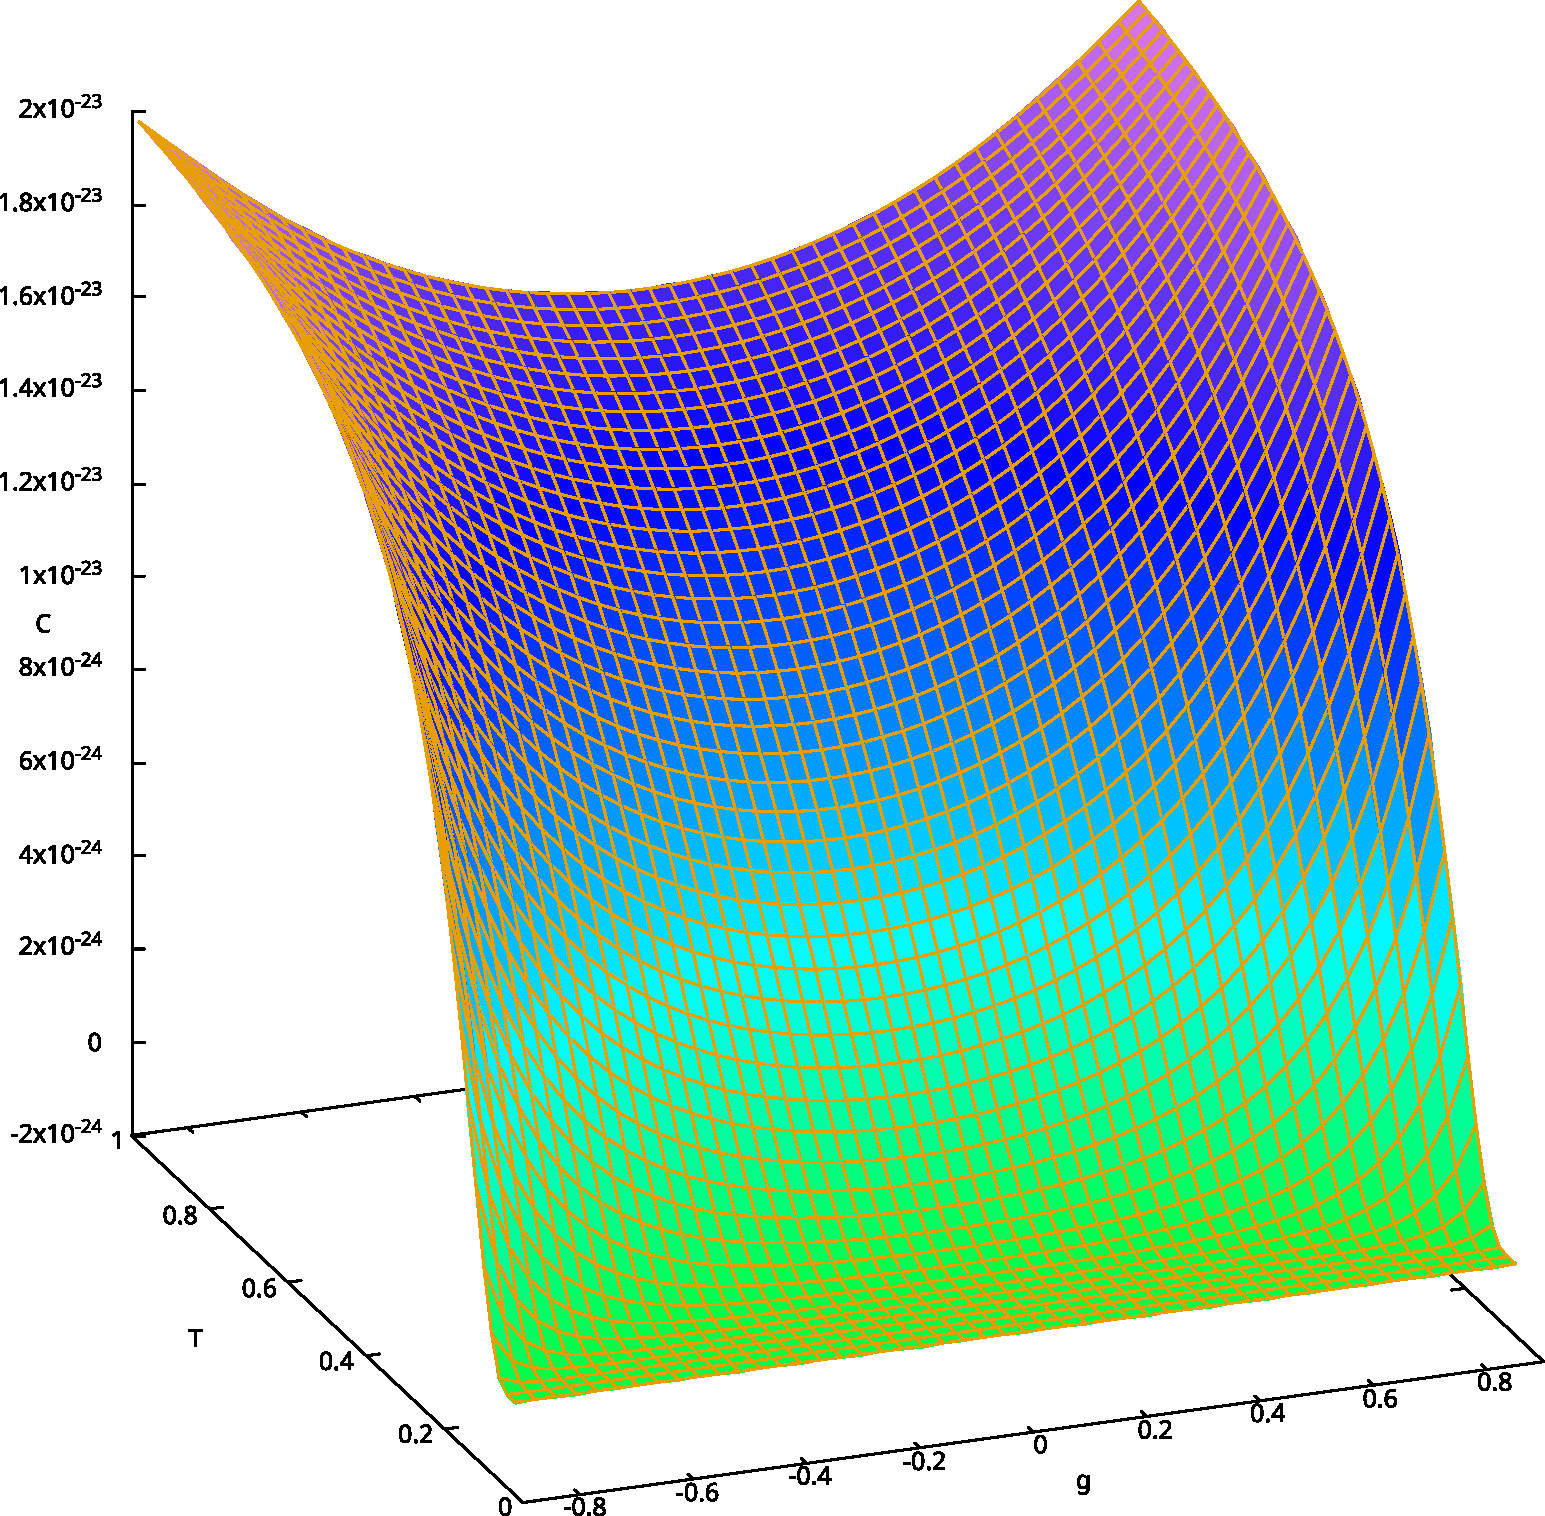
\includegraphics[width=\textwidth]{maxima/m1a1b1T0_1S400_2.pdf}
    \caption{Soojusmahtuvuse sõltuvus gravitatsioonivälja tugevusest ja temperatuurist tükiti lineaarse potentsiaali korral, kus $a=\SI{1}{N}$, $b=\SI{1}{N}$, $m=\SI{1}{kg}$ ja $N=400$.}
    \allikas{Autori erakogu.}
    \label{joon1}
\end{figure}

Joonis \ref{joon5} erineb joonisest \ref{joon1} b väärtuse poolest.
On näha, et üldine kuju on mõlemal juhul sama.
Joonise \ref{joon5} jaoks on sümmeetriatelg nihutatud.
Tõenäoliselt on sümmeetriatelg alati $g$ sellise väärtuse juures, kus potentsiaal \eqref{linpot} on sümmeetriline nullpunkti suhtes.
Võrrandist \eqref{linpot} on lihtne näha, et sümmeetria esineb, kui
\begin{equation}
    a-mg=b+mg
\end{equation}
ehk
\begin{equation}
    g=\frac{a-b}{2m}.
\end{equation}

\begin{figure}[htb!]
    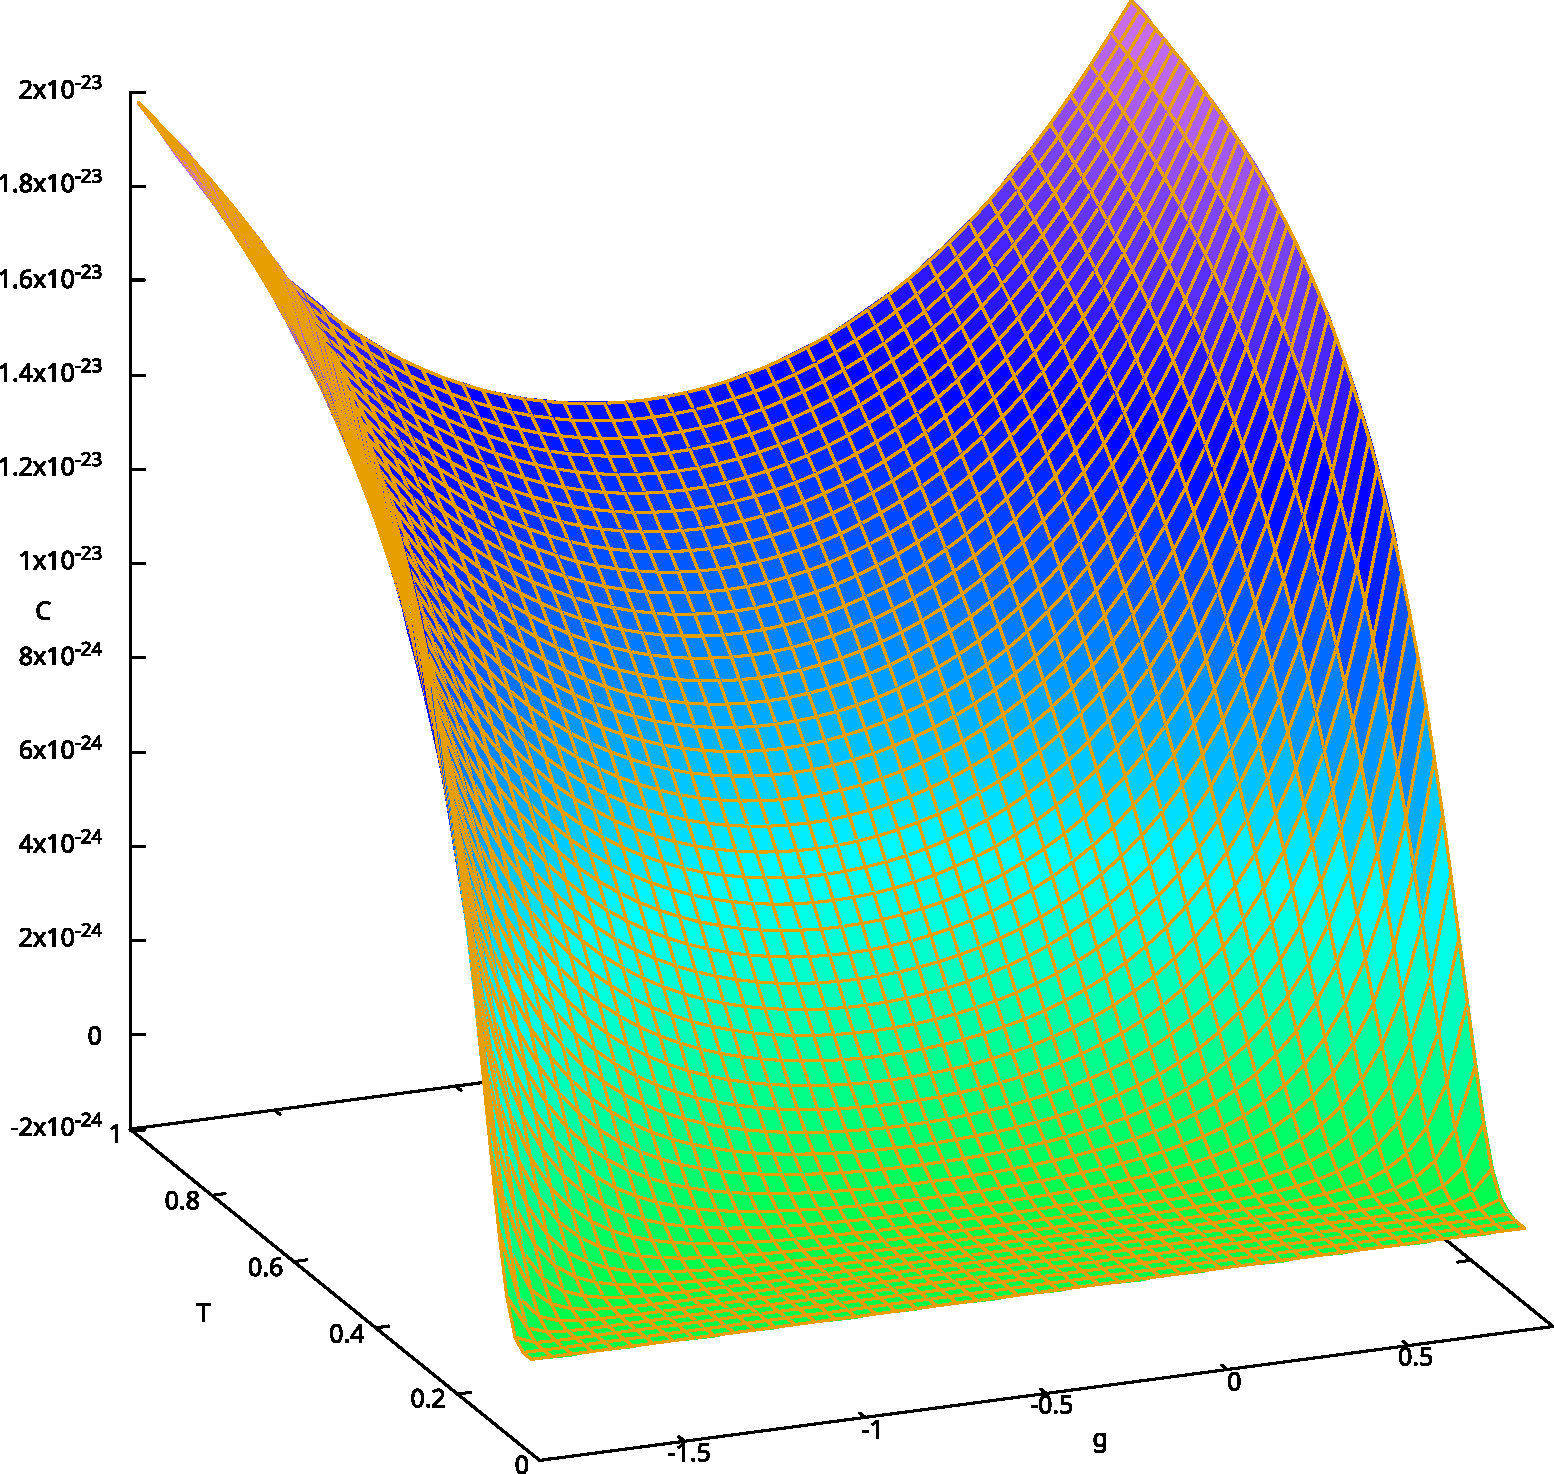
\includegraphics[width=\textwidth]{maxima/m1a1b2T0_1S400.pdf}
    \caption{Soojusmahtuvuse sõltuvus gravitatsioonivälja tugevusest ja temperatuurist tükiti lineaarse potentsiaali korral, kus $a=\SI{1}{N}$, $b=\SI{2}{N}$, $m=\SI{1}{kg}$ ja $N=400$.}
    \allikas{Autori erakogu.}
    \label{joon5}
\end{figure}

Joonised \ref{joon3} ja \ref{joon4} erinevad ainult summeeritud liikmete arvu poolest.
On näha mõlemal joonisel, et madalatel temperatuuridel on soojusmahtuvus väike, tõustes mingi väärtuseni ja siis hakates sümmeetriateljest kaugemal vähenema.
Kuna maksimaalne väärtus on mõlemal juhul ligikaudu sama avaldise \eqref{intmahtuvus} väärtusega, siis tõenäoliselt on sümmeetriateljest kaugemal vähenemine tingitud summeerimise ebatäpsusest ja tegelikult seda ei esine.
Seda väidet kinnitab ka täpsemal joonisel (joonis \ref{joon4}) väiksem soojusmahtuvuse vähenemine sümmeetriateljest kaugemal.

\begin{figure}[htb!]
    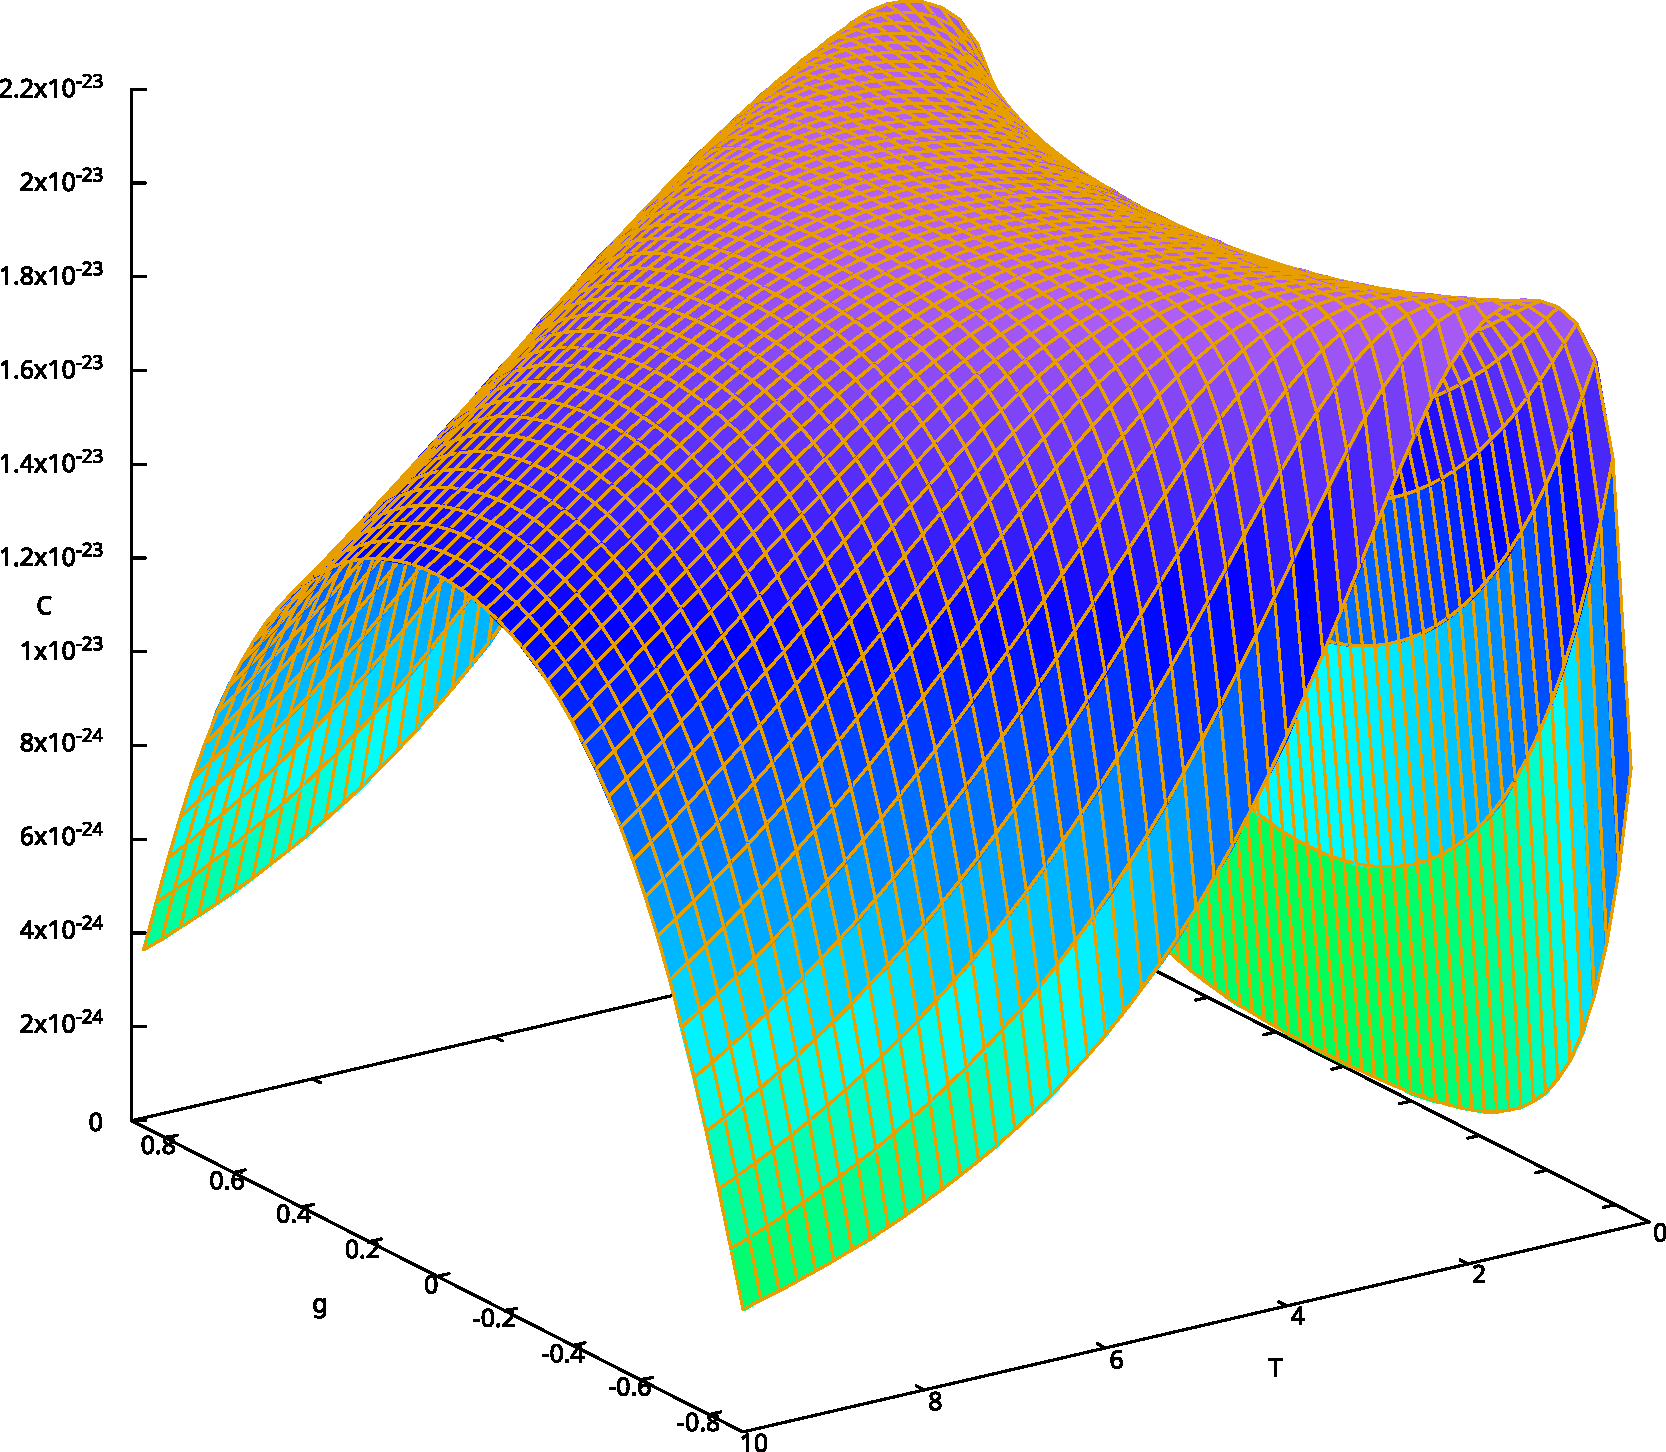
\includegraphics[width=0.6\textwidth]{maxima/m1a1b1T0_10S100.pdf}
    \caption{Soojusmahtuvuse sõltuvus gravitatsioonivälja tugevusest ja temperatuurist tükiti lineaarse potentsiaali korral, kus $a=\SI{1}{N}$, $b=\SI{1}{N}$, $m=\SI{1}{kg}$ ja $N=100$.}
    \allikas{Autori erakogu.}
    \label{joon3}
\end{figure}

\begin{figure}[htb!]
    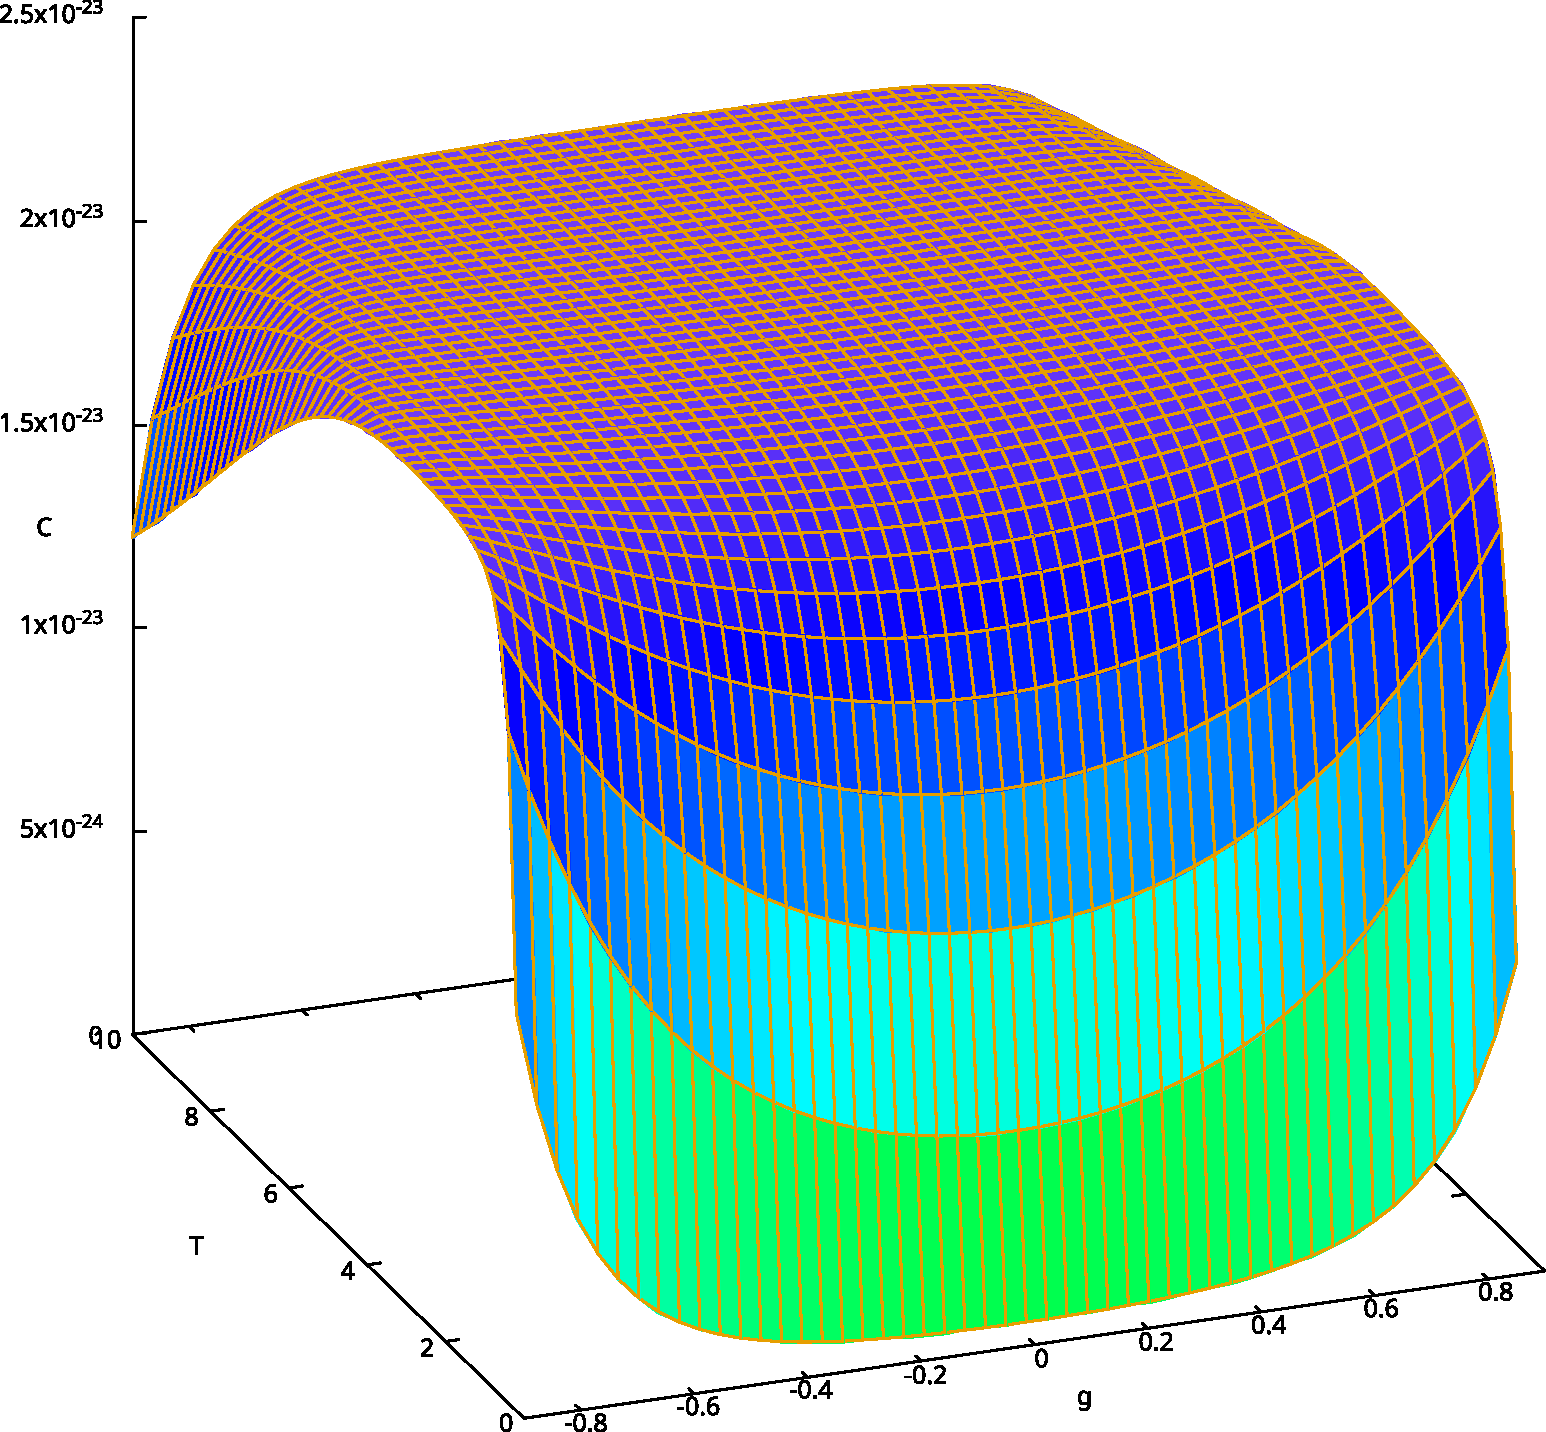
\includegraphics[width=0.6\textwidth]{maxima/m1a1b1T0_10S400.pdf}
    \caption{Soojusmahtuvuse sõltuvus gravitatsioonivälja tugevusest ja temperatuurist tükiti lineaarse potentsiaali korral, kus $a=\SI{1}{N}$, $b=\SI{1}{N}$, $m=\SI{1}{kg}$ ja $N=400$.}
    \allikas{Autori erakogu.}
    \label{joon4}
\end{figure}

%\begin{figure}[htb!]
%    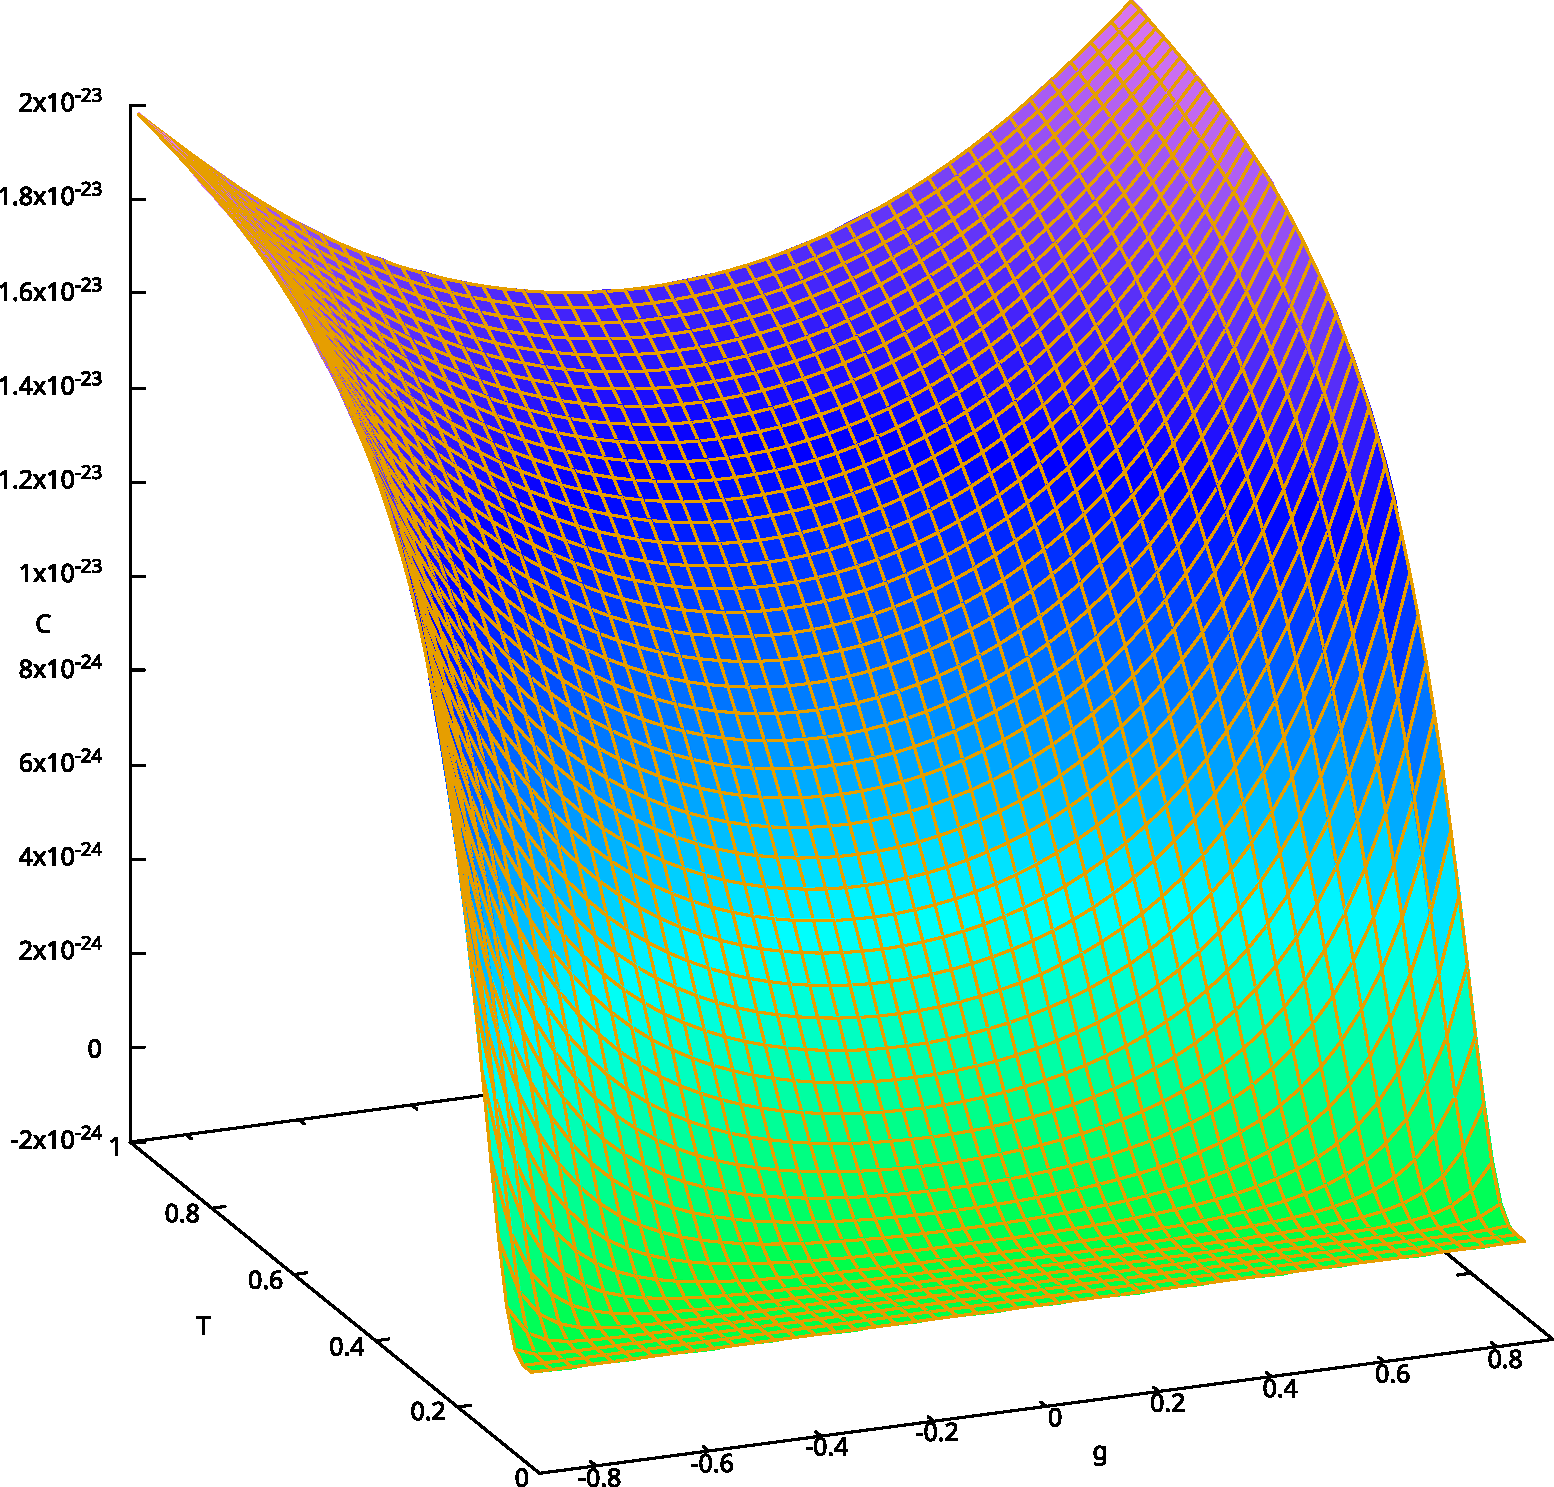
\includegraphics[width=0.7\textwidth]{maxima/m1a1b1T0_1S100.pdf}
%    \caption{Soojusmahtuvuse sõltuvus gravitatsiooniväljast ja temperatuurist tükiti lineaarse potentsiaal korral, kus $a=\SI{1}{N}$, $b=\SI{1}{N}$, $m=\SI{1}{kg}$ ja $N=100$.}
%    \allikas{Autori erakogu.}
%    \label{joon2}
%\end{figure}



%\section{Tükiti paraboolne potentsiaal}
%
%\begin{equation}
%    \frac{\sqrt{m} \left( \sqrt{2} {g}^{2} m^2 + {{2}^{\frac{5}{2}}}\, {E_n} a\right)  \arcsin\left( \frac{\sqrt{{{g}^{2}}\, {{m}^{2}}+4 {E_n} a} \sqrt{{{g}^{2}}\, {{m}^{4}}+4 {E_n} a\, {{m}^{2}}}}{{{g}^{2}}\, {{m}^{3}}+4 {E_n} a m}\right) }{4 {{a}^{\frac{3}{2}}}}=\ensuremath{\pi}  \left( n+\frac{1}{2}\right)  \hbar
%\end{equation}

\section{Häiritusega harmooniline ostsillaator}

Käesolevas osas vaadeltakse harmoonilist ostsillaatorit, millele on lisatud kuuphäiritus, gravitatsiooniväljas.

\subsection{Harmooniline ostsillaator gravitatsiooniväljas}

Selleks, et leida häirituse mõju süsteemile lahendatakse kõigepealt omaväärtusprobleem harmoonilise ostsillaatori jaoks gravitatsiooniväljas.
Järgnev on sarnane tuletuskäiguga tavalise harmoonilise ostsillaatori jaoks, kuid erineb detailide poolest ja seega on siiski siin ära toodud.
Tavalise harmoonilise ostsillaatori jaoks võib leida tuletuskäigu Shankari materjalist \parencite[202-216]{shankar94}.
Gravitatsiooniväljas paiknevale ostsillaatorile vastav hamiltoonian on
\begin{equation}
    \op[0]{H}=\frac{\op{p}^2}{2m}+\frac{m\omega^2 \op{x}^2}{2} + mg\op{x}=\hbar \omega (A^\dagger A + 1/2)-k_1,
\end{equation}
kus $k_1=\frac{mg^2}{2\omega^2}$ ja
\begin{align}
    \begin{split}
        A &= \sqrt{\frac{m\omega}{2\hbar}}\left[ \left( \op{x} + \frac{g}{\omega^2} \right) + \frac{i}{m\omega} \op{p} \right], \\
        A^\dagger &= \sqrt{\frac{m\omega}{2\hbar}}\left[ \left( \op{x} + \frac{g}{\omega^2} \right) - \frac{i}{m\omega} \op{p} \right],
    \end{split}
\end{align}
$A^\dagger$ on $A$ kaasoperaator.
Defineeritakse operaator $\mathcal{H}$ järgnevalt:
\begin{equation}
    \mathcal{H} = \frac{\op[0]{H}}{\hbar \omega}=(A^\dagger A + 1/2)-\frac{k_1}{\hbar \omega}.
    \label{mathcalH}
\end{equation}
Tahetakse leida omaväärtused järgmisele võrrandile:
\begin{equation}
    \mathcal{H}\ket{\varepsilon}=\varepsilon \ket{\varepsilon}.
\end{equation}
Kehtivad järgnevad omadused:
\begin{align}
%    \left[A, A^\dagger\right] &= 1, \\
    \left[A, \mathcal{H}\right] &=A\mathcal{H} - \mathcal{H}A=A, \\
    \left[A^\dagger, \mathcal{H}\right] &= A^\dagger \mathcal{H} - \mathcal{H} A^\dagger = -A^\dagger.
\end{align}
Operaatorid $A$ ja $A^\dagger$ on tekitavad uusi omaseisundeid. Kuna
\begin{align}
        \mathcal{H}A\ket{\varepsilon}&=\left(A\mathcal{H}-[A, \mathcal{H}]\right)\ket{\varepsilon} \nonumber\\
        &=(A\mathcal{H}-A)\ket{\varepsilon} \nonumber\\
        &=(\varepsilon - 1)A\ket{\varepsilon},
\end{align}
siis peab oleama $A\ket{\varepsilon}$ omaseisundeid omaväärtusega $\varepsilon - 1$, st
\begin{equation}
    A\ket{\varepsilon}=C_\varepsilon \ket{\varepsilon -1},
    \label{cepsilon}
\end{equation}
kus $C_\varepsilon$ on konstant ja $\ket{\varepsilon -1}$ ja $\ket{\varepsilon}$ on normeeritud omaketid.
Sarnaselt nähakse, et
\begin{align}
        \mathcal{H}A^\dagger\ket{\varepsilon}&=\left(A^\dagger\mathcal{H}-[A^\dagger, \mathcal{H}]\right)\ket{\varepsilon} \nonumber \\
        &=(A^\dagger\mathcal{H}+A^\dagger)\ket{\varepsilon} \nonumber \\
        &=(\varepsilon + 1)A^\dagger\ket{\varepsilon},
\end{align}
nii et
\begin{equation}
    A^\dagger\ket{\varepsilon}=C_{\varepsilon+1} \ket{\varepsilon+1}.
    \label{cepsilon1}
\end{equation}
Kuna $\mathcal{H}$ omaväärtused ei saa lõputult väheneda, siis peab olema seisund $\ket{\varepsilon_0}$, mida ei saa enam alandada:
\begin{equation}
    A\ket{\varepsilon_0}=0.
    \label{nullseis}
\end{equation}
Korrutades võrrandi \eqref{nullseis} läbi operaatoriga $A^\dagger$ saadakse, et
\begin{equation}
    A^\dagger A\ket{\varepsilon_0}=0.
    \label{aanull}
\end{equation}
Võrranditest \eqref{mathcalH} ja \eqref{aanull} saadakse, et
\begin{equation}
    \left(\mathcal{H}-1/2 + \frac{k_1}{\hbar \omega} \right)\ket{\varepsilon_0}=0
\end{equation}
või
\begin{equation}
    \mathcal{H}\ket{\varepsilon_0}=\left(\frac{1}{2} - \frac{k_1}{\hbar \omega}\right) \ket{\varepsilon_0}
\end{equation}
või
\begin{equation}
    \varepsilon_0=\frac{1}{2} - \frac{k_1}{\hbar \omega}.
\end{equation}
Kasutades operaatorit $A^\dagger$ korduvalt saab suurendada seisundit $\ket{\varepsilon_0}$ lõputult. Seega avalduvad ostsillatori energiatasemed järgnevalt:\footnote{Kuna ühes dimensioonis pole kidumist, siis need on ainsad energiatasemed \parencite[176-177]{shankar94}.}
\begin{equation}
    \varepsilon_n=\left(n+\frac{1}{2}\right)-\frac{k_1}{\hbar \omega}, \qquad n=0, 1, 2,\dots
\end{equation}
või
\begin{equation}
    E_n=\hbar \omega \left(n+\frac{1}{2}\right)-k_1, \qquad n=0, 1, 2,\dots
    \label{nullenergia}
\end{equation}
%Nüüd tahetakse leida võrranditest \eqref{cepsilon} ja \eqref{cepsilon1} konstandid $C_\varepsilon$ ja $C_{\varepsilon+1}$.
Kuna $\varepsilon=n+1/2 - k_1/\hbar \omega$, tähistatakse kette täisarvuga $n$.
Tahetakse leida konstant $C_n$ järgmisest võrrandist:
\begin{equation}
    A\ket{n}=C_n \ket{n -1}.
    \label{konstket}
\end{equation}
Võrrandi \eqref{konstket} kaasvõrrand on
\begin{equation}
    \bra{n}A^\dagger=\bra{n-1}C_n^*.
    \label{konstbra}
\end{equation}
Kombineerides võrrandid \eqref{konstket} ja \eqref{konstbra} saadakse, et
\begin{align}
    \braket{n|A^\dagger A|n}&=\braket{n-1|C_n^* C_n| n-1} \\
    \braket{n|\mathcal{H}-\tfrac{1}{2}+\tfrac{k_1}{\hbar \omega}|n}&=C_n^* C_n \\
    \braket{n|n|n}&=|C_n|^2 \\
    |C_n|^2&=n \\
    C_n&=\sqrt{n} e^{i\phi}.
\end{align}
Kuna $\phi$ väärtus on vabalt valitav, siis on mugav võtta selle väärtus nulliks. Siis saadakse, et
\begin{equation}
    A\ket{n}=\sqrt{n}\ket{n-1}.
\end{equation}
Analoogselt saab näidata, et
\begin{equation}
    A^\dagger \ket{n}=\sqrt{n+1}\ket{n+1}.
\end{equation}

\subsection{Häiritusega harmooniline ostsillaator gravitatsiooniväljas}

Nüüd vaadatakse harmoonilist ostsillaatorit, millele on lisatud kuuphäiritus, gravitatsiooniväljas. Sellele vastav hamiltoniaan on
\begin{equation}
    \op{H}=\op[0]{H}+\op[1]{H},
\end{equation}
kus
\begin{equation}
    \op[1]{H}=\lambda \op{x}^3 = \lambda \left[ \sqrt{\frac{\hbar}{2m\omega}}(A^\dagger + A) - \frac{g}{\omega^2}\right]^3=\lambda \left(\frac{\hbar}{2m\omega}\right)^\frac{3}{2} (A^\dagger + A - k_2)^3,
\end{equation}
kus $k_2=g\sqrt{\frac{2m}{\hbar \omega^3}}$.
Kuna sellele hamiltoniaanile vastava omaväärtusülesande täpselt lahendamine pole tõenäoliselt võimalik, siis kasutatakse häiritusteooriat. Võrrandi \eqref{parand1} järgi on esimene parand omaväärtustele
\begin{equation}
    E_n^1=\braket{n|\op[1]{H}|n}=\lambda \left(\frac{\hbar}{2m\omega}\right)^\frac{3}{2} \braket{n|(A^\dagger + A - k_2)^3|n},
    \label{kuupparand1}
\end{equation}
Kuna $A^\dagger$ ja $A$ muudavad omaseisundit, siis peab olema neid hulkliikme $(A^\dagger + A + k_2)^3$ üksliikmes sama palju, et eelnev avaldis poleks null. Seega annavad avaldises \eqref{kuupparand1} nullist erinevad liikmed ainult üksliikmed $-k_2^3$, $-3k_2A^\dagger A$ ja $-3k_2AA^\dagger$. Järelikult
\begin{align}
    E_n^1&=\lambda \left(\frac{\hbar}{2m\omega}\right)^\frac{3}{2} \braket{n|-k_2^3-3k_2A^\dagger A- 3k_2 A A^\dagger|n} \nonumber \\
    &= -\lambda \left(\frac{\hbar}{2m\omega}\right)^\frac{3}{2} (k_2^3 + 3k_2\sqrt{n}\sqrt{n} + 3k_2\sqrt{n+1}\sqrt{n+1}) \nonumber \\
    &= -\lambda \left(\frac{\hbar}{2m\omega}\right)^\frac{3}{2} [k_2^3 + 3k_2(2n+1)] \label{uksenergia}.
\end{align}
Võrranditest \eqref{nullenergia} ja \eqref{uksenergia} saadakse, et
\begin{equation}
    E_n \approx \left(n+\frac{1}{2}\right) - k_1 - \lambda \left(\frac{\hbar}{2m\omega}\right)^\frac{3}{2} [k_2^3 + 3k_2(2n+1)].
    \label{kuupene}
\end{equation}
Võrranditest \eqref{part} ja \eqref{kuupene} saadakse, et statistiline summa on
\begin{equation}
    Z=\sum_{n=0}^{\infty} \exp\left(-\beta \left(\left(n+\frac{1}{2}\right) - k_1 - \lambda \left(\frac{\hbar}{2m\omega}\right)^\frac{3}{2} (k_2^3 + 3k_2(2n+1)) \right)\right).
\end{equation}
Tegu on geomeetrilise rea summaga. See koondub järgmisel tingimusel:
\begin{equation}
    \frac{3}{\sqrt{2}}k_2\lambda \left(\frac{\hbar}{m\omega}\right)^{\frac{3}{2}}<1
\end{equation}
või
\begin{equation} \label{eeldus}
    3 \lambda \hbar g < m \omega^3.
\end{equation}
Selle eelduse kehtimisel on
\begin{equation}
    Z=\frac{\exp\left( \beta \left(  \lambda (k_2^3+3k_2)\left(\frac{\hbar}{2m\omega}\right)^{\frac{3}{2}} +k_1 -\frac{1}{2}\right)\right)}{1-\exp \left( \beta\left( 6 k_2 \lambda \left( \frac{\hbar}{2m\omega}\right)^{\frac{3}{2}} - 1 \right)\right)}.
\end{equation}
Siit pole raske leida soojusmahtuvuse avaldist, kuid kuna see on küllaltki pikk ja otseselt sellest valemist pole võimalik järeldusi teha, siis ei hakata seda siin välja tooma.

Kasutades Maxima programmi üritas autor teha graafikuid soojusmahtuvuse sõltuvuse kohta temperatuurist ja gravitatsiooniväljast, kuid $\hbar$ ja $k_B$ tegelike väärtuste korral ei õnnestunud luua ühtegi graafikut.
See on tõenäoliselt tingitud sellest, et väärtused lähevad liiga väikseks programmi Maxima jaoks.
Teatud väärtuste (vt joonis \ref{hjoon1} ja \ref{hjoon2}) jaoks õnnestus siiski luua soojusmahtuvuse ja soojusmahtuvuse tuletise gravitatsioonivälja järgi graafikud.
Graafikute tegemisel on arvestatud, et eeldus \eqref{eeldus} kehtiks.
Kuna soojusmahtuvus muutub lubatud $g$ muutumispiirkonnas väga vähe, siis on joonise \ref{hjoon2} usaldusväärsus kaheldav ja võib olla tingitud arvutuslikest ebatäpsustest.


\begin{figure}[htb!]
    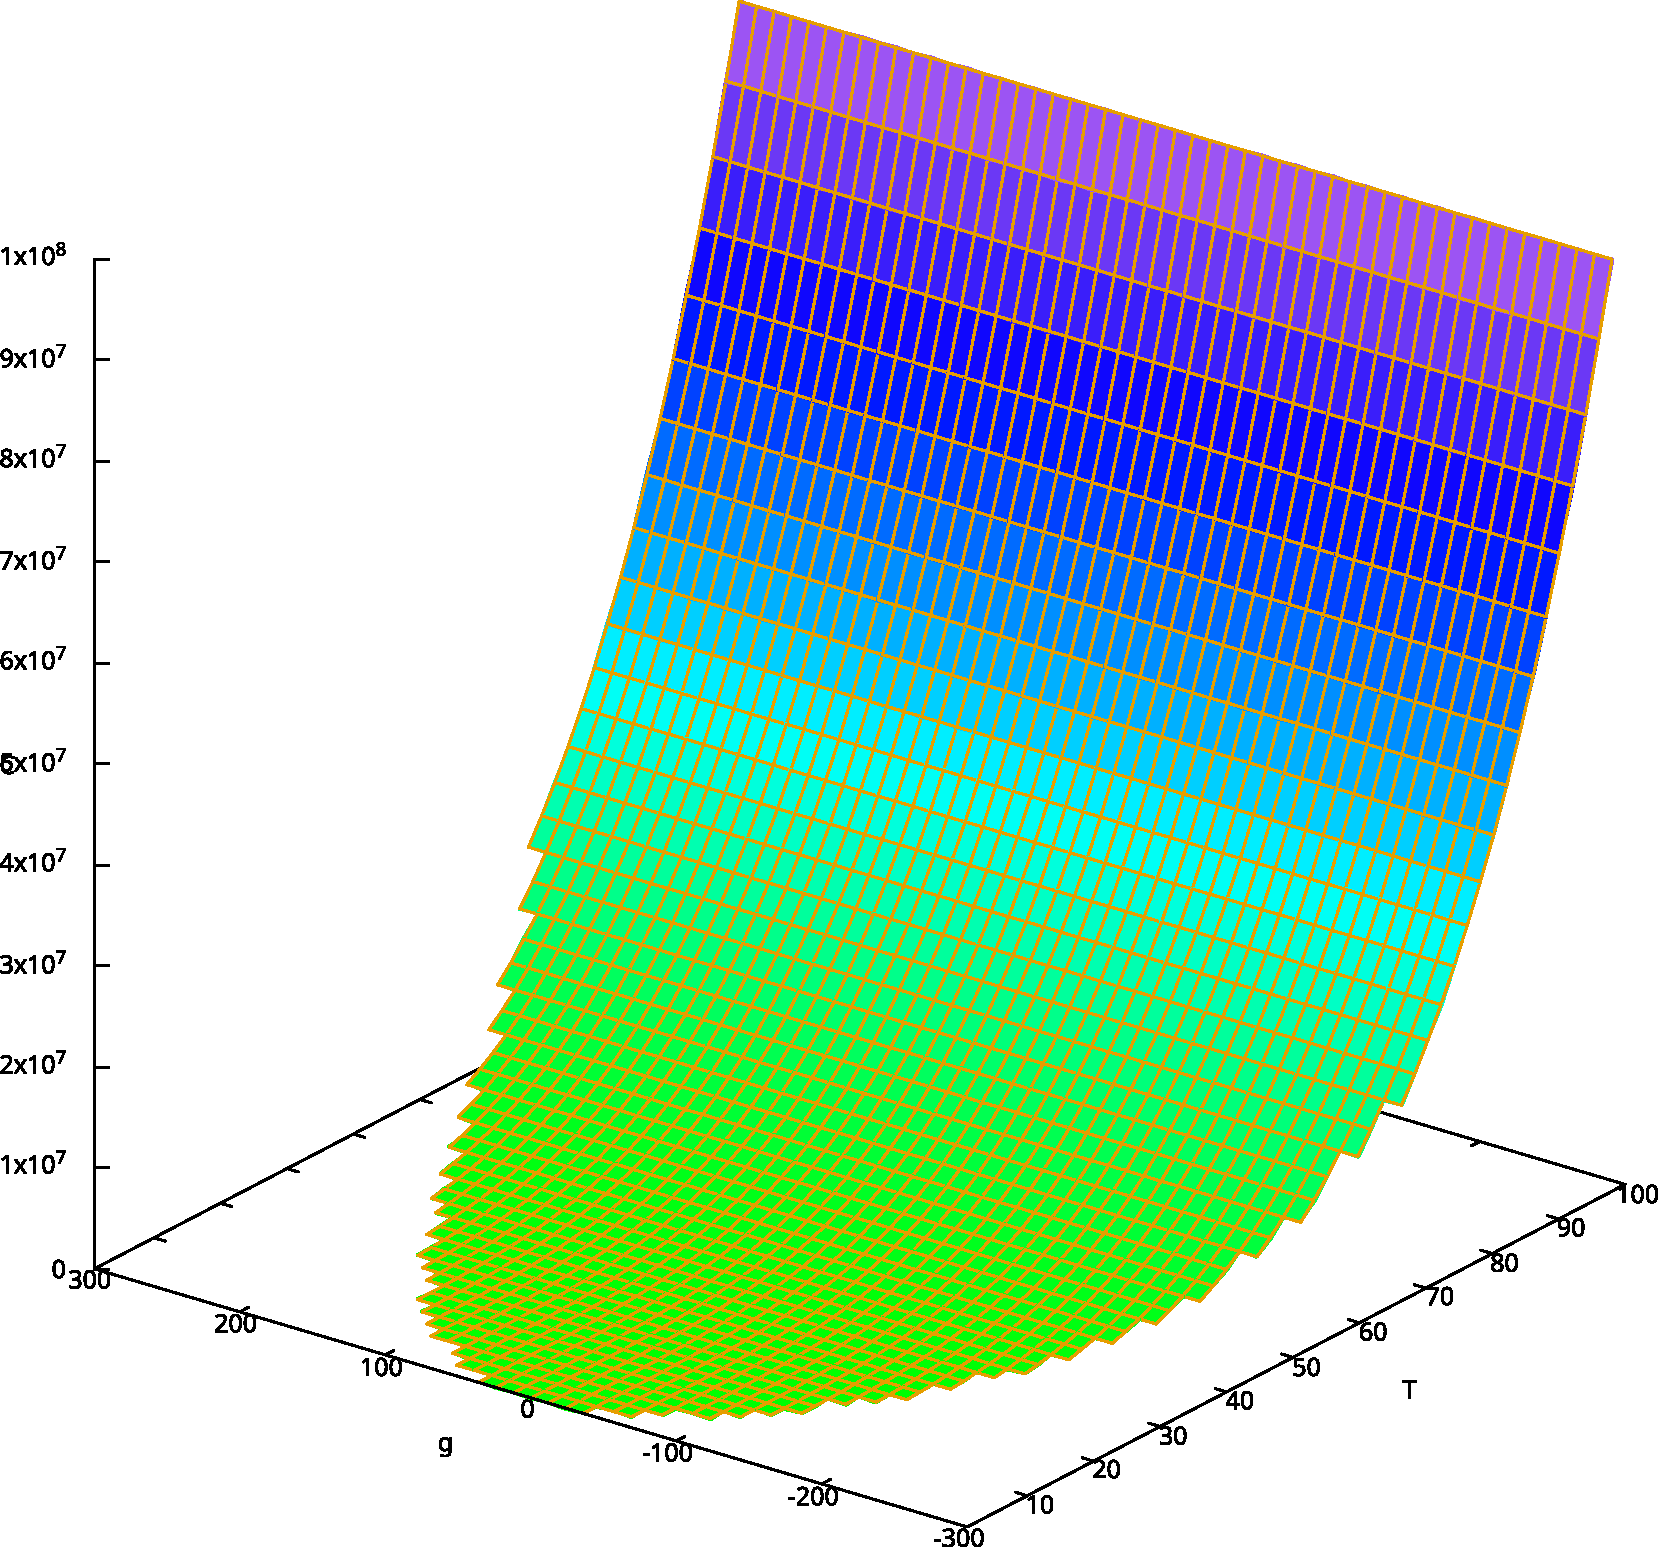
\includegraphics[width=0.6\textwidth]{maxima/harh1k1m1w1l0001.pdf}
    \caption{Soojusmahtuvuse sõltuvus gravitatsioonivälja tugevusest ja temperatuurist häiritusega harmoonilise ostsillaatori jaoks gravitatsiooniväljas, kus $\hbar=\SI{1}{J.s}$, $k_B=\SI{1}{J.K^{-1}}$, $m=\SI{1}{kg}$, $\omega=\SI{1}{s^{-1}}$ ja $\lambda=\SI{1e-3}{J.m^{-3}}$.}
    \allikas{Autori erakogu.}
    \label{hjoon1}
\end{figure}

\begin{figure}[htb!]
    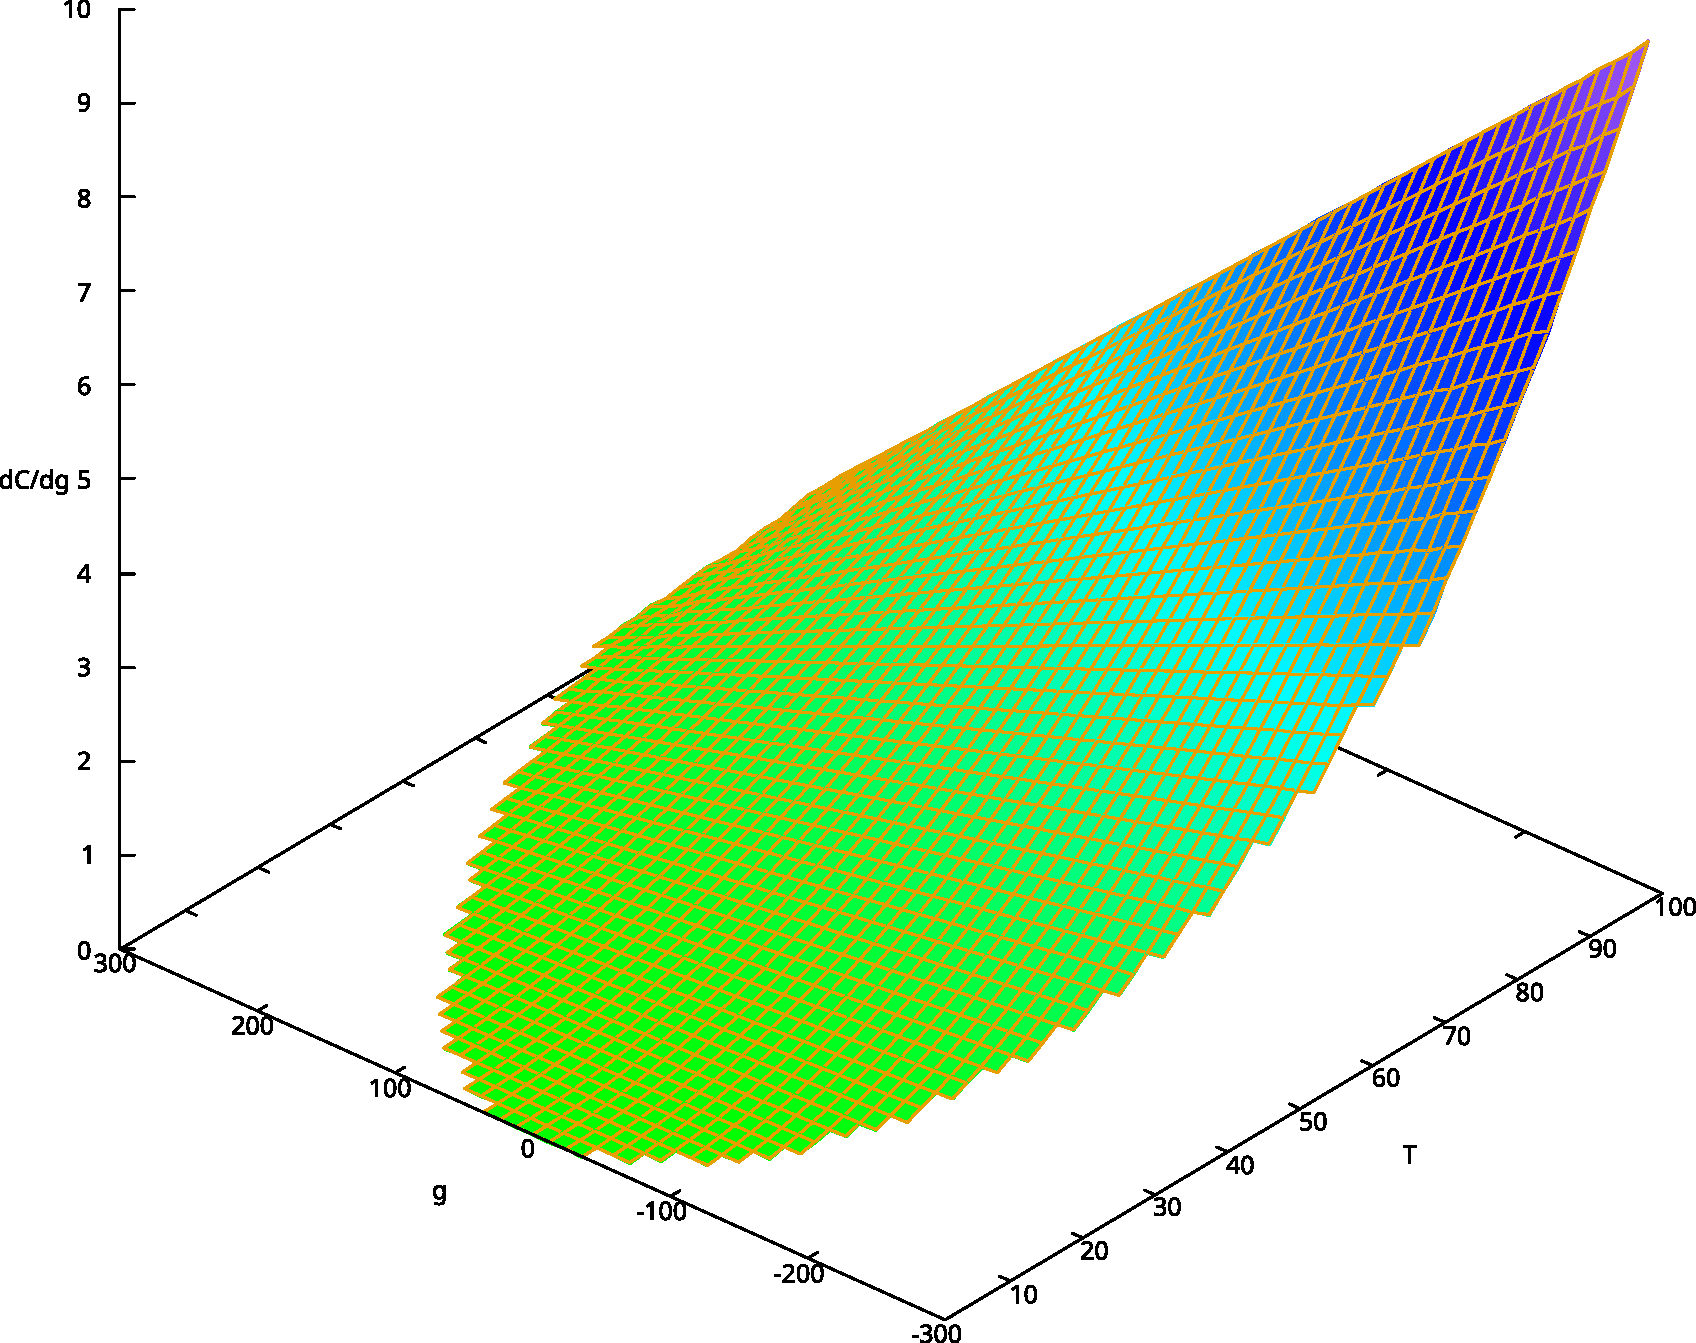
\includegraphics[width=0.6\textwidth]{maxima/dcdgharh1k1m1w1l0001.pdf}
    \caption{Soojusmahtuvuse tuletise gravitatsioonivälja suhtes sõltuvus gravitatsioonivälja tugevusest ja temperatuurist häiritusega harmoonilise ostsillaatori jaoks gravitatsiooniväljas, kus $\hbar=\SI{1}{J.s}$, $k_B=\SI{1}{J.K^{-1}}$, $m=\SI{1}{kg}$, $\omega=\SI{1}{s^{-1}}$ ja $\lambda=\SI{1e-3}{J.m^{-3}}$.} %$\hbar=1$, $k_B=1$, $m=1$, $\omega=1$ ja $\lambda=\num{1e-3}$.}
    \allikas{Autori erakogu.}
    \label{hjoon2}
\end{figure}

%\begin{multline}
%    \frac{2 \left( 6 k_2 \lambda \left(\frac{\hbar}{2m \omega}\right)^\frac{3}{2}-1\right)^{2} \exp\left(\beta  \left( \frac{\left( {{{k_2}}^{3}}+3 {k_2}\right)  \lambda  {{\left( \frac{\hbar }{m \omega }\right) }^{\frac{3}{2}}}}{{{2}^{\frac{3}{2}}}}+ k_1 - \frac{1}{2}\right) +3 \sqrt{2} {k_2} \beta  \lambda  {{\left( \frac{\hbar }{m \omega }\right) }^{\frac{3}{2}}}-2 \beta \right)}{{{\left( 1-{\exp{\frac{3 {k_2} \beta  \lambda  {{\left( \frac{\hbar }{m \omega }\right) }^{\frac{3}{2}}}}{\sqrt{2}}-\beta }}\right) }^{3}}} +\\
%    \frac{\left( \frac{3 {k_2} \lambda  {{\left( \frac{\hbar }{m \omega }\right) }^{\frac{3}{2}}}}{\sqrt{2}}-1\right)  \left( \frac{\left( {{{k_2}}^{3}}+3 {k_2}\right)  \lambda  {{\left( \frac{\hbar }{m \omega }\right) }^{\frac{3}{2}}}}{{{2}^{\frac{3}{2}}}}+\frac{3 {k_2} \lambda  {{\left( \frac{\hbar }{m \omega }\right) }^{\frac{3}{2}}}}{\sqrt{2}}+{k_1}-\frac{3}{2}\right)  {{ e}^{-\beta  \left( -\frac{\left( {{{k_2}}^{3}}+3 {k_2}\right)  \lambda  {{\left( \frac{\hbar }{m \omega }\right) }^{\frac{3}{2}}}}{{{2}^{\frac{3}{2}}}}-{k_1}+\frac{1}{2}\right) +\frac{3 {k_2} \beta  \lambda  {{\left( \frac{\hbar }{m \omega }\right) }^{\frac{3}{2}}}}{\sqrt{2}}-\beta }}}{{{\left( 1-{{ e}^{\frac{3 {k_2} \beta  \lambda  {{\left( \frac{\hbar }{m \omega }\right) }^{\frac{3}{2}}}}{\sqrt{2}}-\beta }}\right) }^{2}}}+ \\
%    \frac{\left( \frac{3 {k_2} \lambda  {{\left( \frac{\hbar }{m \omega }\right) }^{\frac{3}{2}}}}{\sqrt{2}}-1\right)  \left( \frac{\left( {{{k_2}}^{3}}+3 {k_2}\right)  \lambda  {{\left( \frac{\hbar }{m \omega }\right) }^{\frac{3}{2}}}}{{{2}^{\frac{3}{2}}}}+{k_1}-\frac{1}{2}\right)  {{ e}^{-\beta  \left( -\frac{\left( {{{k_2}}^{3}}+3 {k_2}\right)  \lambda  {{\left( \frac{\hbar }{m \omega }\right) }^{\frac{3}{2}}}}{{{2}^{\frac{3}{2}}}}-{k_1}+\frac{1}{2}\right) +\frac{3 {k_2} \beta  \lambda  {{\left( \frac{\hbar }{m \omega }\right) }^{\frac{3}{2}}}}{\sqrt{2}}-\beta }}}{{{\left( 1-{{ e}^{\frac{3 {k_2} \beta  \lambda  {{\left( \frac{\hbar }{m \omega }\right) }^{\frac{3}{2}}}}{\sqrt{2}}-\beta }}\right) }^{2}}}+ \\
%    \frac{{{\left( \frac{\left( {{{k_2}}^{3}}+3 {k_2}\right)  \lambda  {{\left( \frac{\hbar }{m \omega }\right) }^{\frac{3}{2}}}}{{{2}^{\frac{3}{2}}}}+{k_1}-\frac{1}{2}\right) }^{2}} {{ e}^{-\beta  \left( -\frac{\left( {{{k_2}}^{3}}+3 {k_2}\right)  \lambda  {{\left( \frac{\hbar }{m \omega }\right) }^{\frac{3}{2}}}}{{{2}^{\frac{3}{2}}}}-{k_1}+\frac{1}{2}\right) }}}{1-{{ e}^{\frac{3 {k_2} \beta  \lambda  {{\left( \frac{\hbar }{m \omega }\right) }^{\frac{3}{2}}}}{\sqrt{2}}-\beta }}}
%\end{multline}

\section{Järeldused}




\addchap{Kokkuvõte}

Töös leiti ligikaudsed soojusmahtuvuse avaldised kahe kvantmehaanilise süsteemi jaoks.
Tükiti lineaarse potentsiaali jaoks gravitatsiooniväljas õnnestus leida, et väga kõrgetel temperatuuridel ei sõltu soojusmahtuvus gravitatsioonivälja tugevusest. Madalatel temperatuuridel leiti, et potentsiaali sümmeetrilisuse tõttu võib soojusmahtuvus nii tõusta kui ka langeda. Häiritusega harmoonilise ostsillaatori jaoks gravitatsiooniväljas ei leitud küll hästi analüüsitavat tulemust ja soojusmahtuvuse sõltuvus gravitatsioonist on kaheldav, kuid selle eest leiti täpne avaldis statistilise summa jaoks, millest pole raske jõuda soojusmahtuvuse avaldiseni.

Kinnitust sai hüpotees, et on võimalik soojusmahtuvust nii suurendada kui ka vähendada.

Tulemuste leidmine osutus ootamatult keeruliseks.
On väga vähe potentsiaale, mille jaoks on Schrödingeri võrrand analüütiliselt lahenduv.
Autor ei leidnud ühtegi potentsiaali, milles oleks lineaarselt koordinaadist sõltuv osa ja mille jaoks soojusmahtuvus sõltuks gravitatsioonivälja tugevusest.

Edaspidi tasuks uurida sama teemat, aga teistsuguste potentsiaalide jaoks. Kõige lihtsam oleks ilmselt uurida potentsiaale, mis on analüütiliselt lahenduvad ilma gravitatsioonivälja komponendita, häirituse meetodil.

\printbibliography
\addchap{Lisa 1 Maxima kood} \label{maximalisa}
\begin{lstlisting}[language=Maxima, breaklines=true]
(%i1)	E_n: (3^(2/3)*%pi^(2/3)*(g^2*m^2+b*g*m-a*g*m-a*b)^(2/3)*(2*n+1)^(2/3)*hbar^(2/3))/(2^(5/3)*(b+a)^(2/3)*m^(1/3));
(E_n)	(3^(2/3)*%pi^(2/3)*(g^2*m^2+b*g*m-a*g*m-a*b)^(2/3)*(2*n+1)^(2/3)*hbar^(2/3))/(2^(5/3)*(b+a)^(2/3)*m^(1/3))
(%i2)	Z: sum(%e^(-E_n*beta), n, 0, 400)$
(%i3)	diff(log(Z), beta, 1)$
(%i4)	subst(1/(k_B*T), beta, %o3)$
(%i5)	diff(%o4, T, 1)$
(%i6)	C: -%o5$
(%i7)	subst(1,m,C)$
(%i8)	subst(1,a,%o7)$
(%i9)	subst(1,b,%o8)$
(%i10)	subst(1.38064852e-23,k_B,%o9)$
(%i11)	subst(1.054571800e-34,hbar,%o10)$
(%i12)	plot3d(%o11, [g,-0.9,0.9], [T,0,1], [grid, 50, 50], [zlabel, "C"], [gnuplot_pm3d,true]);
\end{lstlisting}

\addchap{Abstract}
\addchap{Resümee}
%\kinnitusleht

\end{document}
